\chapter{统计物理}

\originalpage{257}{242}
迄今为止，我们讨论的问题都是确定性的问题：已知足以描述系统几乎全部行为的信息，求解确定性的方程，以期得到一个确定性的结论。

然而，物理上存在这样一类系统，其中包含着非常庞大的自由度，我们仅知道其很少的一部分整体性质，例如能量、压强、体积等等。不过这些系统总是会进入这样一种状态：这些整体性质不随时间变换，且相互之间满足几乎确定的函数关系。我们将这样的状态称为热平衡态。热平衡态这个概念会牵扯到许多复杂的数学问题，有些直到现在都没有得到完美解决。我们不会去过分纠缠这些基础理论，而仅仅考虑如何在它们成立的情况下求解实际物理问题。

当掌握了处理这类包含大量未知自由度系统的数值方法后，我们会发现它们可以反过来应用于确定性问题。在不少情况下，它们甚至比确定性的算法更有效率，而仅有的缺陷在于，我们无法保证得到的结果一定能够在某个误差范围内等同于真实解，而只能说数值结果以非常高的概率落在误差范围内。

本章中我们将首先由统计物理中的系综的概念引入概率分布，研究如何求解大自由度系统的平衡态，并探讨概率这个概念如何应用于其他确定性问题之上。

\section{系统平均：抽样与蒙特卡洛方法}

我们尝试从热力学的结论来导出统计物理中的一些基本假设。

设某个系统的运动可以由一个 $2n$ 维的哈密顿函数 $H(p,q)$ 描述。除去一些宏观量外，我们并不知道这个系统的细节信息。那么，这个系统的行为原则上应当等于这些细节取遍所有可能性的某种平均。任意物理量 $f(p,q)$ 的期望值写作
\begin{equation}
 \bar f=\frac1N\sum_{i=1}^{N}f(p_i,q_i).
\tag{7.1.1}
\end{equation}
系统的可能状态集合 $\{(p_i,q_i)\}$ 被称为系综（ensemble）。我们可以将前式中的求和改写成积分的形式。为此，引入密度分布
\begin{equation}
 \rho(p,q)=\frac1N\sum_{i=1}^{N}\delta^{(2n)}\!\left[(p,q)-(p_i,q_i)\right].
\tag{7.1.2}
\end{equation}

\originalpage{258}{243}
那么有
\begin{equation}
 \bar f=\int f(p,q)\rho(p,q)\,d^np\,d^nq.
\tag{7.1.3}
\end{equation}
当系统的分布足够稠密时，密度分布 $\rho$ 将从一系列 $\delta$ 函数的求和过渡到连续函数。

当系统处在平衡态时，任何宏观量的期望值都不应当随时间而变化，这相当于要求分布 $\rho(p,q)$ 不随时间变化。而每一个可能状态 $(p_i,q_i)$ 均满足哈密顿方程，是时间的函数。那么，将密度分布对时间取微分，并利用链式法则可以得到
\begin{align}
 \partial_t\rho
 &=\frac1N\sum_{i=1}^{N}
 \left(\dot p_i\partial_{p_i}+\dot q_i\partial_{q_i}\right)
 \delta^{(2n)}\!\left[(p,q)-(p_i,q_i)\right]\notag\\
 &=-\left(\dot p\partial_p+\dot q\partial_q\right)\rho\notag\\
 &=\{H,\rho\}.
\tag{7.1.4}
\end{align}
从中得知分布函数 $\rho$ 与哈密顿函数 $H$ 的泊松括号为零，也就是说 $\rho$ 是一个运动常数。

接下来我们需要借助热力学第零定律的推论：将两个相同温度的系统放在一起做热接触，两个系统的状态都不会改变。这意味着一个大系统的分布函数可以拆分成两个子系统分布函数的乘积：
\begin{equation}
 \rho_{12}=\rho_1\rho_2,
 \qquad
 \ln\rho_{12}=\ln\rho_1+\ln\rho_2.
\tag{7.1.5}
\end{equation}
这是一个非常有趣的结果：$\ln\rho$ 是一个线性可加的运动常数。注意到热接触意味着容许两个系统交换能量，而对于与相互作用相比自能可忽略的两个系统而言，能量也是线性可加的，我们由此可以写下
\begin{equation}
 \ln\rho=\alpha+\beta H(p,q).
\tag{7.1.6}
\end{equation}
这是熟知的 Boltzmann 分布，其中 $\alpha$ 是归一化常数，$\beta$ 是温度的负倒数。

如果我们拓展热接触的定义，容许两个系统交换动量、角动量甚至粒子\footnote{在多数情况下，粒子数是运动常数。例外情形包含化学反应、声子，以及相对论极限下粒子的产生、湮灭等。}，线性可加的运动常数目就变多了，这时的分布函数会写作
\begin{equation}
 \ln\rho=\alpha+\beta H+\bm\gamma\cdot\bm P+\bm\delta\cdot\bm L+\sum_i\mu_i n_i.
\tag{7.1.7}
\end{equation}
两个容许交换动量的系统达到平衡的必要条件是质心速度相等，那么 $\bm\gamma$ 应当正比于系统的质心速度。类似地，可以论证 $\bm\delta$ 和 $\mu_i$ 分别正比于系统的角速度矢量和第 $i$ 类粒子

\originalpage{259}{244}
的化学势。我们可以写下一个更一般的表达式
\begin{equation}
 \rho=\frac1Z e^{\sum_k c_k f_k},
\tag{7.1.8}
\end{equation}
其中 $f_k$ 是某个广延量，而 $c_k$ 为其对偶的强度量，归一化常数 $Z$ 被称为配分函数：
\begin{equation}
 Z=\int e^{\sum_k c_k f_k(p,q)}\,d^np\,d^nq,
\tag{7.1.9}
\end{equation}
可以视作这些强度量的函数。对应广延量的期望值可以通过对配分函数求偏导数得到：
\begin{equation}
 \bar f_i=\frac{\partial\ln Z}{\partial c_i}.
\tag{7.1.10}
\end{equation}

这样，一个热力学系统的求解归结为计算配分函数。但问题在于，这个 $2n$ 维的积分几乎是不可能解析或者数值计算的，因为问题的维度太高了。为了解决这个问题，我们选择退而求其次，考虑生成一组满足分布 $\rho$ 的系统，从中随机抽取有限个样本来近似替代整个系统，按照 (7.1.1) 式来给出对宏观量 $\bar f$ 的估计。这种通过随机抽样来获得问题的近似解的方法被称为蒙特卡洛（Monte Carlo, MC）方法。

随后的问题便是，如何从给定的分布来获得抽样，这也是本节的主题。

\subsection{随机数产生器}

最基础，也是最简单的问题，是如何生成 $[0,1)$ 区间上的均匀分布 $U(0,1)$：
\begin{equation}
 \rho(x)=
 \begin{cases}
 1,&0\le x<1,\\
 0,&\text{其他情况}.
 \end{cases}
\tag{7.1.11}
\end{equation}
显然，随手取 $n$ 个等距点
\begin{equation}
 x_i=\frac{i-1/2}{n},\qquad i=1,2,\ldots,n,
\tag{7.1.12}
\end{equation}
这些点在该区间分布非常均匀。然而，这样的采样通常是不能用的，因为我们希望采样获得的一系列点 $\{x_i\}$ 符合独立同分布（independent and identically distributed, IID）。不同的采样点之间不能有任何的关联。这会便于后续处理更复杂的问题。

这就把人给难住了。计算机上运行的都是确定性的程序，怎么才能生成一系列独立的、随机的数据呢？在大多数时候，人们同样选择退一步：让不同样本之间的关联足够反常，以至于在绝大多数实际情况中无法影响最终的数值结果。这样生成的样本被称为伪随机数（pseudo random number）。

一个常用的产生伪随机数的方法是 Lehmer 所提出的线性同余法：
\begin{equation}
 x_{n+1}=(ax_n+c)\bmod m,\qquad n=0,1,2,\ldots,
\tag{7.1.13}
\end{equation}

\originalpage{260}{245}
其中 $x_0,a,c,m$ 都是正整数，$x_0$ 被称为随机数种子（seed）。这个递归关系给出了一个数列，取值范围为 $0$ 至 $m-1$ 间的任意整数。由于其定义了一个有限集合中的单向映射，产生的数列一定是循环的。一个好的线性同余法需要恰当选取 $a$ 和 $c$ 的值，使得循环周期达到其最大值 $m$。GCC 标准库中的取法为
\begin{equation}
 m=2^{31},\qquad a=1103515245,\qquad c=12345,
\tag{7.1.14}
\end{equation}
其循环周期为 $m$。其余编程语言中的一些取法可以在网络上找到。在得到 $0$ 至 $2^{31}-1$ 上的均匀采样后，再将它们除以 $2^{31}$ 就能够得到浮点精度下 $[0,1)$ 区间上的均匀分布 $U(0,1)$。

我们说过，一个理想的伪随机数发生器应当让不同样本之间的关联足够反常，难以被发现。然而线性同余法生成的数列中存在着一个明显的关联。Marsaglia 指出\footnote{Marsaglia G. Random numbers fall mainly in the planes. \emph{Proc. Natl. Acad. Sci.}, 1968, 61: 25.}，令线性同余数列中连续 $s$ 个数据代表 $s$ 维空间中的一个点 $(x_{i+1},x_{i+2},\ldots,x_{i+s})$，那么这些点将分布在不多于 $(s!m)^{1/s}$ 个相互平行的超平面上。对于 $m=2^{31}$，取 $s=28$，可以得到这些点将分布在不超过 24 个相互平行的超平面上，相比于真正的独立同分布产生的 $m^s$ 种可能性，线性同余法生成的全部可能点集所占的比例仅为 $24/m\sim10^{-8}$。因此，当面临高维度问题时，线性同余法并不是一个足够好的伪随机数产生器。

\begin{exerciseBox}[练习 7.1]
取 $m=2^{31},a=7,c=0$，编程实现线性同余随机数产生器。分别画出 $\{x_n/m\}$ 的分布直方图以及 $(x_i,x_{i+1})$ 的二维散点图，解释你的结果。
\end{exerciseBox}

另一个常用的方案是 Tausworthe 所提出的反馈移位寄存器。这个随机数产生器的实现需要存储之前所产生过的 $n$ 个随机数，递归公式为
\begin{equation}
 X_i=X_{i-p}\oplus X_{i-q},
\tag{7.1.15}
\end{equation}
其中符号 $\oplus$ 代表二进制数的按位异或操作。恰当选取整数 $p,q$，使对应的二元域特征多项式为本原多项式时，这类伪随机数产生器的周期可以达到 $2^{\max\{p,q\}}-1$；一个常见的取法为 $p=250,q=103$。\jiaokan{原印本称“整数 $p,q$ 满足 $p^2+q^2+1$ 为素数”即可得到最长周期。反馈移位寄存器取得最大周期的关键条件并非这一算术条件，而是相应的特征多项式在 $\mathrm{GF}(2)$ 上为本原多项式；原条件一般不足以保证最大周期。}

反馈移位寄存器生成的数列中同样存在微妙的关联，并且会导致求解某些物理问题时数值结果出现错误。我们将在 7.3 节的最后再次提到这件事。

\subsection{直接抽样法}

当我们获得了由 $U(0,1)$ 生成的抽样 $\xi$ 后，我们可以将其转换成任意一维区间 $[a,b]$

\originalpage{261}{246}
上分布密度函数 $\rho(x)$ 的抽样。引入分布函数
\begin{equation}
 F(x)\equiv\int_a^x\rho(x')\,dx',
\tag{7.1.16}
\end{equation}
代表依照 $\rho(x)$ 取样时，样本落在区间 $[a,x]$ 中的概率。它与 $\xi$ 落在 $[0,F(x)]$ 中的概率是一致的。那么，我们可以推断
\begin{equation}
 \eta=F^{-1}(\xi)
\tag{7.1.17}
\end{equation}
给出了区间 $[a,b]$ 上分布密度函数 $\rho(x)$ 的抽样。这种方法被称为直接抽样法。

直接抽样法可用的前提是积分以及反函数 $F^{-1}$ 可以解析给出或容易数值得到。我们来看一个简单的例子。考虑 $[0,\infty)$ 上的分布 $\rho(x)=\alpha e^{-\alpha x}$，那么
\begin{equation}
 F(x)=\int_0^x\alpha e^{-\alpha x'}\,dx'=1-e^{-\alpha x},
\tag{7.1.18}
\end{equation}
则 $\eta=-\ln(1-\xi)/\alpha$ 给出了所需要的抽样。

对于某些特殊的分布密度函数，分布函数无法直接解析给出，但是可以通过别的办法处理。我们来考察实轴 $(-\infty,+\infty)$ 上的高斯分布
\begin{equation}
 \rho(x)=\frac1{\sqrt{2\pi}}\exp\!\left(-\frac{x^2}{2}\right),
\tag{7.1.19}
\end{equation}
它的不定积分无法解析表示。不过，可以回忆一下最初是如何计算它的定积分的：考虑二重积分
\begin{align}
 \int_{-\infty}^{\infty}\rho(x)\,dx\int_{-\infty}^{\infty}\rho(y)\,dy
 &=\frac1{2\pi}\iint\exp\!\left(-\frac{x^2+y^2}{2}\right)dxdy\notag\\
 &=\frac1{2\pi}\iint\exp\!\left(-\frac{r^2}{2}\right)r\,dr\,d\theta,
\tag{7.1.20}
\end{align}
将直角坐标转换成极坐标，原本不能算的积分就成了可以解析计算的了。

我们可以将 $\rho(x)\rho(y)$ 看成一个二维分布密度函数，通过坐标变换，它可以写成两个独立的一维分布密度函数的乘积：
\begin{equation}
 \left\{
 \begin{aligned}
 \rho_r(r)&=\exp\!\left(-\frac{r^2}{2}\right)r,&&r\in[0,\infty),\\
 \rho_\theta(\theta)&=\frac1{2\pi},&&\theta\in[0,2\pi),
 \end{aligned}
 \right.
\tag{7.1.21}
\end{equation}
而它们的分布函数都容易给出解析的积分表达式。那么，我们可以由 $U(0,1)$ 给出两个抽样 $\xi,\eta$ 来得到二维平面 $(r,\theta)$ 上的一个抽样点：
\begin{equation}
 \left\{
 \begin{aligned}
 r&=\sqrt{-2\ln(1-\xi)},\\
 \theta&=2\pi\eta.
 \end{aligned}
 \right.
\tag{7.1.22}
\end{equation}

\originalpage{262}{247}
剩下的便是转换到直角坐标 $(x,y)$ 了：
\begin{equation}
 \left\{
 \begin{aligned}
 x&=\sqrt{-2\ln(1-\xi)}\cos(2\pi\eta),\\
 y&=\sqrt{-2\ln(1-\xi)}\sin(2\pi\eta).
 \end{aligned}
 \right.
\tag{7.1.23}
\end{equation}
$x,y$ 分别给出了两个相互独立的高斯分布抽样，这被称为 Box--Muller 方法。

借助这些结果，我们便可以对一些简单的单粒子或近独立热力学系统进行抽样了。例如，处在重力场中的理想气体的哈密顿量为
\[
 H=\frac{p^2}{2m}+mg\cdot r,
\]
其分布便是一个高斯分布与指数分布的直接乘积。

\subsection{舍选法}

对于更复杂的实际问题中面临的分布密度函数，直接抽样并不总是可行的，我们需要在数值上更一般化的抽样方法。von Neumann 所提出的舍选抽样法（acceptance-rejection sampling）便是一例。

设分布密度函数的定义域有限，$|b-a|<\infty$，且在定义域中不大于 $\lambda$，那么，我们可以先生成 $[a,b]$ 上的均匀抽样
\begin{equation}
 x=a+(b-a)\xi_1,
\tag{7.1.24}
\end{equation}
然后以概率 $\rho(x)/\lambda$ 选择是否接受这个抽样：具体而言，就是再由 $U(0,1)$ 生成一个抽样 $\xi_2$，判断是否满足 $\lambda\xi_2<\rho(x)$。若是，则选择接受 $x$；否则重新抽样 $\xi_1$。这样生成的 $x$ 便是我们所需要的抽样。

舍选法适用于任意复杂的分布密度函数，但是对于某些分布较为极端的函数取样效率较低：其接受率为 $1/(\lambda|b-a|)$，如果区间长度和分布密度的极值都很大，那么通常需要抽样很多次才能得到一个可接受的抽样。此外，对于区间或分布密度函数无界的情形，也无法使用舍选法。为了克服这个困难，人们对舍选法进行了改进。

设我们有另一个 $[a,b]$ 区间\footnote{对于无界区间的情形，后续论述同样适用。}上的概率密度分布 $h(x)$，其抽样可以通过其他方法简单给出。将目标分布密度函数 $\rho(x)$ 做分解
\begin{equation}
 \rho(x)=\lambda\frac{\rho(x)}{\lambda h(x)}h(x)=\lambda g(x)h(x),
\tag{7.1.25}
\end{equation}
其中 $\lambda\ge\max[\rho(x)/h(x)]$。由 $h(x)$ 生成抽样 $\eta$，再由 $U(0,1)$ 生成抽样 $\xi$，若有
\begin{equation}
 \xi<g(\eta),
\tag{7.1.26}
\end{equation}

\originalpage{263}{248}
成立，则接受 $\eta$，否则重新抽样。

这样，抽样值落在 $(\eta,\eta+d\eta)$ 间且被接受的微分概率为
\begin{equation}
 h(\eta)d\eta\times g(\eta)=\frac1\lambda\rho(\eta)d\eta,
\tag{7.1.27}
\end{equation}
为我们所需要的分布。取样的接受率为 $1/\lambda$，通过恰当地选取 $h(x)$ 可以将这个量提高到接近于一。

\subsection{复合抽样法}

舍选抽样法先找到一个随机数，然后再根据第二个随机数判断它是不是需要的抽样。我们也可以将这个过程反过来，根据第一步的随机数判断第二步该如何抽样。这就是复合抽样法，由下式给出：
\begin{equation}
 u(x)=\int v(x|y)w(y)\,dy.
\tag{7.1.28}
\end{equation}
它代表一个两步事件：第一步以概率 $w(y)dy$ 得到随机变量 $\xi$ 位于 $y$ 到 $y+dy$ 之间，第二步以条件概率 $v(x|y)dx$ 得到随机变量 $\eta$ 位于 $x$ 到 $x+dx$ 之间。如果我们不去管 $\xi$，单看 $\eta$，那么它将按照概率密度函数 $u(x)$ 分布。

最典型的复合抽样法为加分布复合抽样。在 $[0,1]$ 区间上取一系列递增的分点
\begin{equation}
 0=F_0<F_1<F_2<\cdots<F_n=1,
\tag{7.1.29}
\end{equation}
令 $w(y)$ 为 $U(0,1)$，并定义条件概率密度
\begin{equation}
 v(x|y)=\sum_{i=1}^{n}f_i(x)\Theta(y-F_{i-1})\Theta(F_i-y),
\tag{7.1.30}
\end{equation}
其中 $f_i(x)$ 为某个概率密度分布函数。$v(x|y)$ 代表着当 $y$ 在 $F_{i-1}$ 和 $F_i$ 之间时，按照概率密度分布 $f_i(x)$ 采样。这样最终可以生成
\begin{equation}
 u(x)=\sum_{i=1}^{n}(F_i-F_{i-1})f_i(x).
\tag{7.1.31}
\end{equation}
换言之，我们可以对不同概率密度分布的加和进行采样。

将舍选抽样法与复合抽样法相组合，我们可以得到相当多复杂概率密度分布的抽样办法。

\subsection{数值积分}

我们之所以讨论了这么长篇幅的抽样，最终目的还是在于计算配分函数的积分。一个 $2n$ 维的积分无论如何都是很困难的，因此我们从一维积分开始讨论。

\originalpage{264}{249}
考察一维积分
\begin{equation}
 I=\int_a^b f(x)\,dx,
\tag{7.1.32}
\end{equation}
$I/(b-a)$ 可以诠释成区间 $[a,b]$ 上均匀分布的随机变量 $x$ 的函数 $f(x)$ 的平均值。因此我们可以用有限个抽样的平均值来近似。

\begin{algorithmBox}[算法 7.1\quad 平均值算法]
\[
 I\approx\frac{b-a}{N}\sum_{i=1}^{N}f(x_i).
\]
\end{algorithmBox}

得到近似方法后，我们自然要问这个近似有多好，为此需要证明两个定理。第一个定理关于单个随机变量偏离其平均值的概率：设随机变量 $x$ 满足概率分布 $\rho(x)$，其平均值和方差分别记作 $\bar x$ 和 $\sigma_x^2$，据定义，
\begin{align}
 \sigma_x^2
 &=\int_a^b(x-\bar x)^2\rho(x)\,dx\notag\\
 &\ge\left[\int_a^{\bar x-\epsilon}+\int_{\bar x+\epsilon}^{b}\right](x-\bar x)^2\rho(x)\,dx\notag\\
 &\ge\epsilon^2\left[\int_a^{\bar x-\epsilon}+\int_{\bar x+\epsilon}^{b}\right]\rho(x)\,dx\notag\\
 &\ge\epsilon^2\Pr(|x-\bar x|>\epsilon).
\tag{7.1.33}
\end{align}
也就是说，随机变量与其平均值相差大于 $\epsilon$ 的概率不高于 $(\sigma_x/\epsilon)^2$。随后将这个结论推广到多个随机变量的代数平均：考虑 $N$ 个满足相同分布的独立随机变量，其代数平均 $\sum_{i=1}^{N}x_i/N$ 构成了一个新的随机变量。其平均值与 $\bar x$ 相等，而方差
\begin{equation}
 \overline{\left(\frac1N\sum_{i=1}^{N}(x_i-\bar x)\right)^2}
 =\sum_{i,j}\frac{\overline{(x_i-\bar x)(x_j-\bar x)}}{N^2}
 =\frac{\sigma_x^2}{N}
\tag{7.1.34}
\end{equation}
会降低为原本的 $1/N$ 倍，其中我们用到了各个 $x_i$ 之间相互独立。这样，如果我们用代数平均来估计平均值 $\bar x$，其与目标值差距大于 $\epsilon$ 的概率将低于 $(\sigma_x/\epsilon)^2/N$。这个结果被称为 \ChebName 大数定律。

我们进一步假设，概率低于某个阈值 $q$ 的小概率事件在实践中几乎不会发生。那么，在绝大多数情况下，$N$ 点代数平均估计平均值的误差
\begin{equation}
 \epsilon<\frac{\sigma_x}{\sqrt{Nq}}.
\tag{7.1.35}
\end{equation}

\originalpage{265}{250}
按照 $N^{-1/2}$ 的速度收敛于零。这个结果显然要比在 2.2 节和 3.5 节中介绍过的任何数值积分方法都差远了。但是，我们需要注意到，上面的证明其实并不依赖于问题的维度：对于任意维度的积分，基于随机变量方法的误差总是依 $O(N^{-1/2})$ 的速度趋于零，而对于基于网格划分的积分方法，在 $d$ 维空间中的 $N$ 个格点对应每个维度上仅有 $N^{1/d}$ 个格点，其误差的收敛速度将从一维情况下的 $O(N^{-s})$ 降低至 $O(N^{-s/d})$。只要问题维度足够高，MC 方法总会展现出它的优势。此外，MC 方法对于被积函数的解析性质没有任何要求，这也是它相对格点划分方法的优势之一。

MC 方法的误差除了正比于 $N^{-1/2}$ 外，同时也正比于统计量的标准差 $\sigma$。对于一维积分而言，它的方差为
\begin{equation}
 \sigma_f^2=\frac1{b-a}\int_a^b[f(x)-\bar f]^2\,dx,
\tag{7.1.36}
\end{equation}
如果能够降低统计量的方差，那么积分精度也能得到提高。为此，与舍选法类似，我们可以将函数 $f(x)$ 做分解：
\begin{equation}
 f(x)=\frac{f(x)}{h(x)}h(x)=g(x)h(x),
\tag{7.1.37}
\end{equation}
其中 $h(x)$ 为 $[a,b]$ 区间上的概率密度分布，且容易进行采样。这样，定积分变成了 $g(x)$ 在概率密度分布 $h(x)$ 下的平均值，由下式近似给出：
\begin{equation}
 I\approx\frac1N\sum_{i=1}^{N}g(x_i),
\tag{7.1.38}
\end{equation}
其中 $x_i$ 由概率密度分布 $h(x)$ 生成。如果我们能通过恰当地选取 $h(x)$ 使得 $g(x)$ 接近于一个常函数，从而其方差足够小，那么 MC 方法求积分的精度也将会很高。这个思想被称为重要性抽样（importance sampling）。

最极端的情形是 $g(x)$ 为常函数，我们只需要一个采样点就能得到精确的积分结果
\begin{equation}
 I=g(x),
\tag{7.1.39}
\end{equation}
不过，这也意味着原被积函数 $f(x)$ 等于一个已知的概率密度分布乘上一个常数，其积分结果本来就是已知的。

\begin{exerciseBox}[练习 7.2]
自行设计抽样方案，使用 MC 方法计算积分
\[
 I=\int_1^\infty e^{-x^2/2}\,dx.
\]
\end{exerciseBox}

如何恰当选取和生成 $h(x)$ 以减小 MC 方法的误差是一个非常重要的课题。人们发展了所谓自适应技术，根据已经得到的部分抽样结果来反复改进 $h(x)$，从而逼近最

\originalpage{266}{251}
优概率密度分布\footnote{感兴趣的读者可以参考综述 Arouna B. Adaptative Monte Carlo method, a variance reduction technique. \emph{Monte Carlo Method Appl.}, 2004, 10(1): 1.}。

我们再来谈谈多维积分的问题。如果积分区域相对规则，可以在某个坐标系下写成多维度直积的形式
\begin{equation}
 \omega=[a_1,b_1]\otimes[a_2,b_2]\otimes\cdots\otimes[a_d,b_d].
\tag{7.1.40}
\end{equation}
那么对于格点方法而言，可以在每个维度上各取一组网格，然后直接计算。但对于不少现实问题来说，我们只能给出关于积分区域的一个隐函数表达式
\begin{equation}
 p(x_1,x_2,\ldots,x_d)>0,
\tag{7.1.41}
\end{equation}
并且 $p$ 未必有显式的表达式以及很好的解析性质，此时要划分网格就很困难了。但对于 MC 方法而言，我们可以选取一个更大的积分区域 $\Omega$，使得 $\omega\subset\Omega$，将积分改写成如下形式：
\begin{equation}
 \int_\Omega f(x)\Theta[p(x)]\,d^dx,
\tag{7.1.42}
\end{equation}
其中 $\Omega$ 是一个相对规则的区域。由于 MC 方法不依赖于被积函数的解析性质，额外附加的阶跃函数不会显著影响其精度。注意，一个高维度区域“体积”的绝大部分都会集中在其边界附近的薄薄一层中，因此 $\Omega$ 的选取必须谨慎。我们也可以采用恰当的重要性抽样，使得抽样点绝大多数都落在区域 $\omega$ 内。

\subsection{拟随机数}

我们重新审视 MC 方法计算数值积分的核心：(7.1.34) 式的推导。借助多次抽样统计独立的性质，它们的代数平均的方差是原本的 $1/N$。如果我们抛弃统计独立这一假设，而认为不同“随机数”之间是负相关的，
\begin{equation}
 \sum_{i\ne j}\overline{(x_i-\bar x)(x_j-\bar x)}<0,
\tag{7.1.43}
\end{equation}
那么其代数平均的方差将会更小，这样可以提高 MC 方法计算数值积分的效率。

负相关意味着不同样本倾向于不待在一起。对于 $N=2$ 的情形，这代表当 $x_1<\bar x$ 时，$x_2$ 就有大概率大于 $\bar x$。这使得它们在实轴上分布得更均匀，那么更高的积分精度也是自然的。这类强调均匀性而忽视关联性的随机数被称为拟随机数（quasi-random number），又称作低差异序列（low-discrepancy sequence）。相应的 MC 方法被称为拟蒙特卡洛（quasi-MC, qMC）方法。在适当的低差异构造及正则性条件下，其误差可接近 $O(N^{-1})$，一般情形则带有依赖维数的对数因子，例如 $O((\log N)^d/N)$。\jiaokan{原印本概括为“其精度通常能够达到 $O(1/N)$ 或 $O(\log N/N)$”。高维低差异序列的经典误差界通常含有依赖维数的对数因子，不能普遍写成与维数无关的 $O(\log N/N)$。}

\originalpage{267}{252}
随意找一个人让他来随机写下一串数，他生成的很可能也是某种拟随机数：因为人总是会避免相近的数连续出现，以及已经多次出现过的数再次出现。不过，如何让计算机来生成满意的拟随机数，这也并不是一个简单的问题。目前常用的算法背后往往都涉及复杂的数论知识。此外，在多维空间生成随机采样时，并不能直接使用一维拟随机数发生器产生的连续若干个序列，而需要专门设计生成拟随机数组的算法\footnote{感兴趣的读者可以参考相关专著 Dick J and Pillichshammer F. \emph{Digital Nets and Sequences: Discrepancy Theory and Quasi-Monte Carlo Integration}. Cambridge University Press, 2010.}。

\subsection{讨论与小结}

本节我们从统计物理中对配分函数的计算出发，引入了蒙特卡洛方法，并介绍了一些基本的生成随机抽样的方法。由于相当一部分物理问题的解都可以归结为某个复杂函数在高维空间中的积分，因而 MC 方法在求解实际物理问题中的应用相当广泛，而不仅仅限于在热力学系统中求解配分函数。本章的后续几节也将继续对 MC 方法展开更深入的讨论。

\section{制备系统：\rusname{Марков} 链}

在上一节中，我们花费了大量篇幅介绍了如何设计算法对任意给定的概率密度分布进行抽样，以及如何通过随机抽样来做数值积分。然而，我们并没有涉及任何统计物理中的例子。这是因为我们实际上并不完全知道一个统计物理系统的概率密度分布。比方说，我们需要对玻尔兹曼分布计算配分函数
\begin{equation}
 Z=\int e^{-\beta H}.
\tag{7.2.1}
\end{equation}
按照重要性抽样的思想，我们需要对 $e^{-\beta H}/Z$ 进行抽样，这样就有
\begin{equation}
 Z=\frac1N\sum_{i=1}^{N}Z_i.
\tag{7.2.2}
\end{equation}
可以发现，我们又绕回到 $Z$ 上面来了。实际上，由于必须知道 $Z$ 的具体大小才能确定玻尔兹曼分布，目前我们甚至无从得知如何对其进行抽样。

我们知道，一个热力学系统经过足够长时间的演化，总会趋向于平衡态，那么我们能否来模拟这一过程呢？换言之，如果我们有一个任意的初态 $x_0$，并通过复合抽样定义条件概率 $q(x_{k+1}|x_k)$，以概率性地给出系统的演化，那么系统的分布将按
\begin{equation}
 f_{k+1}(x)=\int q(x|y)f_k(y)\,dy
\tag{7.2.3}
\end{equation}

\originalpage{268}{253}
做演化。当 $k\to\infty$ 时，$f_k(x)$ 能否趋向于我们所需要的分布 $g(x)$ 呢？

若上述假设成立，我们可以构造相对简单的复合抽样 $q(\cdot|\cdot)$ 来实现玻尔兹曼分布 $\exp(-\beta H)/Z$，那么抽样问题就解决了。如果当 $n>k$ 时，$f_n(x)$ 已经充分接近 $g(x)$，那么随机变量 $x_{k+1},x_{k+2},\ldots$ 都几乎满足同一个分布 $g(x)$（尽管它们通常是高度关联的），我们就能够用它们的平均来计算所需要的热力学量。

这类根据上一步的抽样结果 $x_k$ 来获得当前抽样 $x_{k+1}$ 的随机过程被称为 \rusname{Марков} 过程（Markov process），所生成的随机序列 $\{x_1,x_2,\ldots\}$ 被称为 \rusname{Марков} 链（Markov chain）。其特征是无记忆性，即确定 $x_{k+1}$ 时与 $x_{k-1},x_{k-2},\ldots$ 是多少不直接相关。

为此，让我们在本节中对 \rusname{Марков} 链的性质进行简要的介绍。

\subsection{\rusname{Марков} 过程的性质}

设系统的全体可能状态构成集合 $\Omega$。我们来考察 \rusname{Марков} 过程中会出现什么特殊情况。首先，系统状态集合中可能存在某个只进不出的子集 $\omega$，使得
\begin{equation}
 P(x_{k+1}\in\omega/\Omega\mid x_k\in\omega)=0,\qquad
 P(x_{k+1}\in\omega\mid x_k\in\omega/\Omega)>0.
\tag{7.2.4}
\end{equation}
这样，从某个状态 $x\in\omega/\Omega$ 出发，存在非零的概率让它再也无法回到初始状态。我们称这样的状态是非常返态。反之，如果从某状态出发，经过充分多步后总能回到该状态，我们称其为常返态。全部状态都是常返态的 \rusname{Марков} 过程被称为常返的。

其次，两个子集之间可能完全互不连通：
\begin{equation}
 P(x_{k+1}\in\omega/\Omega\mid x_k\in\omega)=0,\qquad
 P(x_{k+1}\in\omega\mid x_k\in\omega/\Omega)=0.
\tag{7.2.5}
\end{equation}
这个时候我们完全可以将其视作两个独立系统各自的 \rusname{Марков} 过程。我们将这种情况称为可约的。相反，如果从任意状态出发，经过充分多步后总能以非零概率到达另一状态，那么我们将其称为不可约 \rusname{Марков} 过程。

除此之外，特殊形式的转移概率也可能让系统的概率分布做周期振荡。让我们来设想一个两态的 \rusname{Марков} 过程，从 $j$ 态到 $i$ 态的转移概率 $p_{ij}$ 用矩阵形式写作
\begin{equation}
 \mathbf P=
 \begin{pmatrix}
 0&1\\
 1&0
 \end{pmatrix},
\tag{7.2.6}
\end{equation}
显然，其所产生的概率分布将在两个状态之间来回切换。

\originalpage{269}{254}
\subsection{首达概率与线性代数方程组}

让我们来研究 \rusname{Марков} 过程的首达性。为方便表述，以离散系统为例。设系统具有 $n+1$ 个不同的状态，从 $i$ 态一步到 $j$ 态的概率为 $p_{ij}$，满足
\begin{equation}
 p_{ij}\ge0,\qquad \sum_{j=1}^{n+1}p_{ij}=1,
\tag{7.2.7}
\end{equation}
那么，系统从 $i$ 出发，经历一条特定路径 $I$，首次到达 $n+1$ 态这个事件发生的概率为
\begin{equation}
 f(I)=p_{ii_1}p_{i_1i_2}\cdots p_{i_{k-1}i_k}p_{i_kn+1},
\tag{7.2.8}
\end{equation}
对全体路径求和得到
\begin{equation}
 \sum_I f(I)=\sum_{k=0}^{\infty}\sum_{i_1,i_2,\ldots,i_k\ne n+1}
 p_{ii_1}p_{i_1i_2}\cdots p_{i_{k-1}i_k}p_{i_kn+1},\qquad i_0=i.
\tag{7.2.9}
\end{equation}
如果我们将上式中诸如 $p_{i_li_{l+1}}$ 这种看作 $n\times n$ 矩阵 $\mathbf P$，而最后一项 $p_{i_kn+1}$ 看作一个列向量 $\bm p$，则上式可以写成
\begin{equation}
 \sum_I f(I)=\sum_{k=0}^{\infty}\bm e_i^{\mathrm T}\mathbf P^k\bm p
 =\bm e_i^{\mathrm T}(\mathbf I-\mathbf P)^{-1}\bm p.
\tag{7.2.10}
\end{equation}
上述等式中出现了矩阵逆乘向量，也就是线性代数方程组 $(\mathbf I-\mathbf P)\bm x=\bm p$ 的解。这提示我们可以通过 \rusname{Марков} 过程的首达概率来求解线性代数方程组。具体而言，对于 $n$ 阶线性代数方程组，
\begin{equation}
 \mathbf A\bm x=\bm b,
\tag{7.2.11}
\end{equation}
依照 3.2 节的知识，我们可以构造一个收敛的迭代格式
\begin{equation}
 \bm x=\mathbf B\bm x+\bm d,
\tag{7.2.12}
\end{equation}
从而方程的解可以表示为
\begin{align}
 \bm x&=(\mathbf I-\mathbf B)^{-1}\bm d=\sum_{k=0}^{\infty}\mathbf B^k\bm d,\notag\\
 x_i&=\sum_{k=0}^{\infty}\sum_{i_1=1}^{n}\sum_{i_2=1}^{n}\cdots\sum_{i_k=1}^{n}
 b_{ii_1}b_{i_1i_2}\cdots b_{i_{k-1}i_k}d_{i_k}.
\tag{7.2.13}
\end{align}
与之前 $f(I)$ 的形式类似。如果我们可以构造出权重 $w_{ij}$ 和转移概率 $p_{ij}$ 满足
\begin{equation}
 b_{ij}=w_{ij}p_{ij},\qquad d_i=w_{i,n+1}p_{i,n+1},\qquad i,j=1,2,\ldots,n,
\tag{7.2.14}
\end{equation}

\originalpage{270}{255}
其中 $p_{ij}$ 正定归一，那么我们相当于利用 \rusname{Марков} 过程构造出了首达路径的一个概率分布，使得路径依赖的统计量
\begin{equation}
 h(I)=w_{ii_1}w_{i_1i_2}\cdots w_{i_{k-1}i_k}w_{i_kn+1}
\tag{7.2.15}
\end{equation}
在该概率分布下的期望值恰好等于待求的线性代数方程组的解。基于这个思想的算法被称为随机游走方法，计算流程如下。

\begin{algorithmBox}[算法 7.2\quad 随机游走方法]
\begin{enumerate}[label=\arabic*.,leftmargin=2em]
\item 对于线性代数方程组 $\mathbf A\bm x=\bm b$，构造迭代格式 $\bm x=\mathbf B\bm x+\bm d$。构造转移概率 $p_{ij}$ 满足
\[
 p_{ij}=\begin{cases}
 >0,&(j\ne n+1\ \&\&\ b_{ij}\ne0)\ \Vert\ (j=n+1\ \&\&\ d_i\ne0),\\
 0,&\text{其他情况},
 \end{cases}
 \qquad
 \sum_{j=1}^{n+1}p_{ij}=1,
\]
以及相应的权重 $w_{ij}$。
\item 随机游动步数 $k=0$，初始状态 $i_0=i$。
\item 以概率 $p_{i_ki_{k+1}}$ 抽样确定 $i_{k+1}$。
\item 若 $i_{k+1}\ne n+1$，则 $k=k+1$，返回第 3 步。
\item 计算统计量 $h(I)$。
\item 重复 $m$ 次第 2 到 5 步，计算统计平均作为方程的解：
\[
 x_i\approx\frac1m\sum_I h(I).
\]
\end{enumerate}
\end{algorithmBox}

该方法可以逐个地给出方程组的解，因此当我们仅对特定的几个 $x_i$ 感兴趣的时候，通过随机游走模型求解是有优势的。

随机游走方法本质上也是一种蒙特卡洛方法，其误差由下式给出：
\begin{equation}
 \delta\sim\frac{\sigma(h)}{\sqrt m},
\tag{7.2.16}
\end{equation}
与方程的阶数和稀疏程度等因素没有直接联系，适用于高维问题。为减小误差，应尽量减小 $\sigma(h)$ 的值。一个可行的方法是使得全体 $w_{ij}$ 都大致相等，但具体操作并没有统一的策略。

上一节的最后，我们介绍了拟随机数产生器。而数值实验证明\footnote{Mascagni M and Karaivanova A. What are quasirandom numbers good for anything besides integration. \emph{Proceedings of Advances in Reactor Physics and Mathematics and Computation into the Next Millennium (PHYSOR2000)}, 2000.}，在这个问题上使用拟随机数最高可以给出 $O[(\log m)^T/m]$ 的收敛速度，其中 $T$ 为平均路径长度。

\originalpage{271}{256}
\subsection{实例：机器猫和玩具鼠}

舒幼生的《力学》教材中讨论了一个典型的 \rusname{Марков} 过程：如图 7.1 所示，在 $y$ 坐标轴的原点 $O$ 处有一个不动的玩具鼠，在 $y=1$ 处有一个机器猫。机器猫在 $y$ 轴上分别以 $q$ 的概率朝向 $O$ 点，或以 $1-q$ 的概率背离 $O$ 点一步一步行走，步长恒定为 $|\Delta y|=1$。规定猫到达 $O$ 点“捉到”鼠，游戏结束，否则将继续下去。试求机器猫捉到玩具鼠的概率。

\begin{figure}[htbp]
\centering
\begin{tikzpicture}[x=1.7cm,y=1cm,>=Latex]
  \draw[->,thick] (-0.35,0)--(2.65,0) node[right]{$y$};
  \foreach \x/\lab in {0/$O$,1/$1$,2/$2$}{
    \draw (\x,0.06)--(\x,-0.06);
    \node[below=2pt] at (\x,0) {\lab};
  }
  \node[above=6pt] at (0,0) {鼠};
  \node[above=6pt] at (1,0) {猫};
  \fill (0,0) circle (1.8pt);
  \fill (1,0) circle (1.8pt);
\end{tikzpicture}
\caption{猫鼠游戏}
\label{fig:cat-mouse-game}
\end{figure}

这个问题可以抽象为一个 \rusname{Марков} 过程的首达概率问题。记机器猫走了 $k$ 步后处在格点 $y=i$ 的概率为 $z_i^{(k)}$，它可以完全由 $\{z_i^{(k-1)}\}$ 决定：
\begin{equation}
\left\{
\begin{aligned}
 z_0^{(k)}&=qz_1^{(k-1)},\\
 z_1^{(k)}&=qz_2^{(k-1)},\\
 z_i^{(k)}&=(1-q)z_{i-1}^{(k-1)}+qz_{i+1}^{(k-1)},\qquad i\ge2.
\end{aligned}
\right.
\tag{7.2.17}
\end{equation}
也就是说，这一步的概率分布完全由上一步的概率分布给出，是一个 \rusname{Марков} 过程。转移概率为
\[
 p_{ij}=(1-q)\delta_{i-1,j}+q\delta_{i+1,j}.
\]
而机器猫捉到玩具鼠的概率也正好和 $y=1$ 到 $y=0$ 的首达概率在定义上是一致的。因此，我们可以借助前文所给出的 \rusname{Марков} 过程与线性代数方程组的等价性，来求解这个问题。

在这个问题中，我们无须引入任何权重 $w$，从而有 $\bm d=(q,0,0,\ldots)^{\mathrm T}$，以及
\[
\mathbf B=\begin{pmatrix}
0&1-q&&&\\
q&0&1-q&&\\
& q&0&\ddots&\\
&&\ddots&\ddots&\ddots
\end{pmatrix}
\]
均为无穷维向量或矩阵，对应于方程组 $(\mathbf I-\mathbf B)\bm x=\bm d$：
\begin{equation}
\left\{
\begin{aligned}
 x_1-(1-q)x_2&=q,\\
 -qx_1+x_2-(1-q)x_3&=0,\\
 -qx_2+x_3-(1-q)x_4&=0,\\
 &\ \vdots
\end{aligned}
\right.
\tag{7.2.18}
\end{equation}

\originalpage{272}{257}
这里 $x_i$ 便给出了机器猫从 $y=i$ 点出发，最终能抓到玩具鼠的概率。这个无穷维线性代数方程组类似于一个二阶递归数列，具有通解
\begin{equation}
 x_i=1-c\left[1-\left(\frac{q}{1-q}\right)^i\right],
\tag{7.2.19}
\end{equation}
其中 $c$ 为任意常数。这个额外的 $c$ 源自矩阵 $\mathbf I-\mathbf B$ 是一个不满秩的奇异矩阵。由于 $x_i$ 代表一个概率，须满足 $x_i\in[0,1]$，那么当 $q>1/2$ 时，$c$ 只能取零。对于 $q=1/2$ 的临界情形，$c$ 的取值不会影响 $x_i$ 的具体大小。这样我们可以给出
\[
 x_i=1,\qquad q\ge\frac12;
\]
此时机器猫一定能够抓到玩具鼠。

$q<1/2$ 的情形会略微复杂一些。此时从条件 $x_i\in[0,1]$ 出发只能给出 $c\in[0,1]$，没法完全确定问题的解。为此，我们需要重新回到无穷求和式 (7.2.13)。定义
\begin{equation}
 \bm x^{(m)}\equiv\sum_{k=0}^{m}\mathbf B^k\bm d
 =\bm d+\mathbf B\bm x^{(m-1)},
\tag{7.2.20}
\end{equation}
那么对于任意满足 $(\mathbf I-\mathbf B)\bm x=\bm d$ 的 $\bm x$，都可以给出
\begin{align}
 \bm x^{(m)}-\bm x&=\mathbf B[\bm x^{(m-1)}-\bm x],\notag\\
 x_i^{(m)}-x_i&=\sum_j p_{ij}[x_j^{(m-1)}-x_j].
\tag{7.2.21}
\end{align}
容易检验，不论 $c$ 取多少，都有 $x_j^{(0)}-x_j<0$。借助转移概率 $p_{ij}$ 的非负性可以归纳证明，对于任意 $m$ 都有 $x_j^{(m)}-x_j<0$ 成立，也就是说当 $m\to\infty$ 时它应当取它所能达到的最小的那个解，即 $c=1$，
\[
 x_i=\left(\frac{q}{1-q}\right)^i,\qquad q<\frac12,
\]
机器猫存在非零概率抓不到玩具鼠。

\begin{exerciseBox}[练习 7.3]
试通过随机游走方法求解方程组 (7.2.18)。
\end{exerciseBox}

\subsection{偏微分方程的边值问题}

知道了如何使用随机游走方法求解线性代数方程组之后，应用于边值问题是直截了当的。设区域 $\Omega$ 中有方程
\begin{equation}
\begin{aligned}
 \hat A u(\bm r)&=f(\bm r),\qquad \bm r\in\Omega,\\
 u(\bm r)&=g(\bm r),\qquad \bm r\in\partial\Omega.
\end{aligned}
\tag{7.2.22}
\end{equation}

\originalpage{273}{258}
经某种离散化（如有限元法）后得到Jacobi 类的迭代格式
\begin{equation}
 u(\bm r_k)=
 \begin{cases}
 \gamma_k\left[\displaystyle\sum_l\alpha_{kl}u(\bm r_l)+\beta_k f(\bm r_k)\right],&\bm r_k\in\Omega,\\[3pt]
 g(\bm r_k),&\bm r_k\in\partial\Omega.
 \end{cases}
\tag{7.2.23}
\end{equation}
此处的求和限于 $\bm r_k$ 周围的格点（从而存在非零的矩阵元）。通常有 $\alpha_{kl}>0,\beta_k>0$，而 $\gamma_k$ 为归一化常数，使得
\begin{equation}
 \sum_l\alpha_{kl}+\beta_k=1.
\tag{7.2.24}
\end{equation}

生成诸系数后，便可选定出发点 $\bm r$ 随机生成路径 $I$：若某步位于 $\bm r_k\in\Omega$ 处，下一步有 $\alpha_{kl}$ 的概率移动到 $\bm r_l$ 处，以及 $\beta_k$ 的概率终止路径。若 $\bm r_k$ 位于边界上，则直接终止路径。

经 $k$ 步终止于某一点 $\bm r_{i_k}\in\Omega$ 后，计算统计量
\begin{equation}
 h(I)=\prod_{j=1}^{k}\gamma_{i_j}f(\bm r_{i_k}).
\tag{7.2.25}
\end{equation}
若终止于边界点 $\bm r_{i_k}\in\partial\Omega$，统计量为
\begin{equation}
 h(I)=\prod_{j=1}^{k-1}\gamma_{i_j}g(\bm r_{i_k}).
\tag{7.2.26}
\end{equation}
$u(\bm r)$ 的函数值便可以通过计算 $h(I)$ 的期望值得到。

对于二阶偏微分方程，往往有 $\beta\sim\Delta x^2\ll1$，从而路径难以终止于边界点以外的点。因此，有另一种生成路径的方案：取 $\gamma_k$ 使得
\begin{equation}
 \sum_l\alpha_{kl}=1.
\tag{7.2.27}
\end{equation}
每条路径都起始于 $\bm r$，终止于边界，而排除了终止于区域内某一点的可能性。统计量为
\begin{equation}
 h(I)=\sum_{n=0}^{k-1}\left[\prod_{j=1}^{n}\gamma_{i_j}\right]\beta_{i_n}f(\bm r_{i_n})
 +\prod_{j=0}^{k-1}\gamma_{i_j}g(\bm r_{i_k}).
\tag{7.2.28}
\end{equation}

我们依旧以二维 Poisson 方程为例，使用方形网格，并采用有限差分，在 5.1 节中已经得到过这个迭代格式了：
\begin{equation}
 u_{i,j}=\left[\frac{2}{h_x^2}+\frac{2}{h_y^2}\right]^{-1}
 \left\{\frac{u_{i+1,j}+u_{i-1,j}}{h_x^2}+\frac{u_{i,j+1}+u_{i,j-1}}{h_y^2}+f_{ij}\right\}.
\tag{7.2.29}
\end{equation}
取 $h_x=h_y=h$，我们有

\originalpage{274}{259}
\begin{equation}
 \alpha_{kl}=\frac14,\qquad \beta_k=\frac{h^2}{4},\qquad \gamma_k=1.
\tag{7.2.30}
\end{equation}
从而随机路径的生成相当于经典的醉汉行走问题，而统计量为
\begin{equation}
 h(I)=\frac{h^2}{4}\sum_{n=0}^{k-1}f(\bm r_{i_n})+g(\bm r_{i_k}),
\tag{7.2.31}
\end{equation}
是相当简单浅显的一个式子。对于 $f=0$ 的特殊情况，$u(\bm r)$ 甚至就是以其为起点出发的随机路径终点的平均值！这从某种程度上印证了调和函数的均值定理。

设求解域尺度为 $O(L)$，网格尺度为 $\Delta x$。根据 Brown 运动的知识，可知路径的平均长度为 $O(L^2/\Delta x^2)$。在单次模拟上，MC 方法也显示了与空间维度无关的特性，适用于求解高维问题。

当求解热方程的初值问题时，若热方程的格林函数已知：
\begin{equation}
 \partial_tG(\bm r,t;\bm r',t')+\hat A G(\bm r,t;\bm r',t')
 =\delta(\bm r-\bm r')\delta(t-t'),
\tag{7.2.32}
\end{equation}
那么可以使用生成抽样 $G(\bm r,\tau;\bm r',0)$ 的办法来决定每两步之间的移动，而不需要事先对问题进行离散化。例如，对于自由空间的热方程而言，Gauß 分布为其对应的格林函数。\jiaokan{原印本此处写作“对于自由空间的泊松方程而言，高斯分布为其对应的格林函数”。自由空间 Poisson 方程的格林函数是相应维数下的 Coulomb/对数核，并非 Gauß 核；结合本段所讨论的热方程传播子，此处应为自由空间热方程。}

当然，绝大多数问题的格林函数我们并不知道，但是对于不少问题，存在着一些生成近似的短时格林函数的策略，这时候 MC 方法就能发挥重要作用。

\section{相变与临界现象：Ising 模型}

上一节我们从生成 Boltzmann 分布的需求出发引入了 \rusname{Марков} 过程，然而在研究其行为的过程中，讨论了通过其所生成的随机路径来求解线性代数方程组。那么，本节就让我们回归主题，详细地介绍怎么生成 Boltzmann 分布，并求解一个具体的物理问题。

\subsection{细致平衡}

第一个问题是 \rusname{Марков} 过程能否收敛到唯一一个稳定分布上。可以证明，只要该 \rusname{Марков} 过程是常返、不可约且非周期的，上述结论即成立。

稳定分布 $g(x)$ 自然是迭代式 (7.2.3) 的不动点：
\begin{equation}
 g(x)=\int q(x|y)g(y)\,dy.
\tag{7.3.1}
\end{equation}
为了寻找这个不动点，我们可以借助统计物理中的概念。\footnote{王梓坤：《随机过程通论（上卷）》。北京：北京师范大学出版社，1996。}

\originalpage{275}{260}
当 Boltzmann 讨论 $H$ 定理时，他证明了系统达到平衡态时所需满足的细致平衡条件
\begin{equation}
 q(y|x)g(x)=q(x|y)g(y),
\tag{7.3.2}
\end{equation}
即系统处在 $x$ 态的概率乘上从 $x$ 态演化到 $y$ 态的概率，等于系统处在 $y$ 态的概率乘上从 $y$ 态演化到 $x$ 态的概率。我们将 (7.3.2) 式代回 \rusname{Марков} 过程的迭代式，借助
\begin{equation}
 \int q(y|x)\,dy=1,
\tag{7.3.3}
\end{equation}
可知 $g(x)$ 确实是一个迭代不动点。

满足细致平衡条件还能使转移算符在以 $g$ 加权的内积下与一个实对称算符相似，从而其本征值为实数；但这本身并不能保证 \rusname{Марков} 链是非周期的，非周期性仍需作为额外条件保证。\jiaokan{原印本在此声称“由满足细致平衡条件的转移概率生成的马尔可夫过程是非周期的”，并将“不存在周期性”等同于“矩阵 $\mathbf Q$ 的全部本征值是实数”。这并不成立：例如两态转移矩阵 $\begin{psmallmatrix}0&1\\1&0\end{psmallmatrix}$ 满足均匀稳态下的细致平衡，但链的周期为 2，且本征值 $\pm1$ 均为实数。细致平衡保证可逆性与实谱，不自动推出非周期性。}

注意到 (7.2.3) 相当于一个线性变换，可以写成矩阵形式
\begin{equation}
 \bm f_{k+1}=\mathbf Q\bm f_k,
\tag{7.3.4}
\end{equation}
我们考虑相似变换
\begin{equation}
 \mathbf Q'=\mathbf P^{-1}\mathbf Q\mathbf P,
\tag{7.3.5}
\end{equation}
其中 $(P)_{xy}\equiv\sqrt{g(x)}\,\delta(x-y)$，这样
\begin{equation}
 (Q')_{xy}=q(x|y)\sqrt{\frac{g(y)}{g(x)}}
 =q(y|x)\sqrt{\frac{g(x)}{g(y)}}=(Q')_{yx}
\tag{7.3.6}
\end{equation}
是一个实对称矩阵。由于相似变换不改变矩阵本征值，以及实对称矩阵的本征值一定是实数，我们完成了关于实谱的证明。

那么，为了构造 \rusname{Марков} 链使得其趋向于一个给定的分布，我们需要选定 $q(x|y)$ 满足
\begin{equation}
 \frac{q(y|x)}{q(x|y)}=\frac{g(y)}{g(x)}.
\tag{7.3.7}
\end{equation}
这个表达式并不依赖于 $g(x)$ 的归一化系数，也就是说我们摆脱了想求配分函数必须先知道配分函数这个逻辑循环。

将 Boltzmann 分布代入上式，我们得到
\begin{equation}
 \frac{q(y|x)}{q(x|y)}
 =\frac{e^{-\beta\mathcal H(y)}}{e^{-\beta\mathcal H(x)}}
 =e^{\beta[\mathcal H(x)-\mathcal H(y)]},
\tag{7.3.8}
\end{equation}
比值等于两态能量之差的指数函数。实现满足上式的条件概率分布并不困难，这里给出一个综合使用舍选法和复合抽样法进行抽样的例子，即 Barker 算法。

\originalpage{276}{261}
\begin{algorithmBox}[算法 7.3\quad Barker 算法]
\begin{enumerate}[label=\arabic*.,leftmargin=2em]
\item 在系统的可能状态集合中定义二元关系：相邻。与状态 $x$ 相邻的状态数目记作 $m(x)$。
\item 从 $x$ 的全体相邻状态中等概率选取 $z$，计算
\[
 P=\frac{m(x)}{m(z)}e^{\beta[\mathcal H(x)-\mathcal H(z)]}.
\]
\item 以概率 $P/(1+P)$ 选择 $y=z$，以概率 $1/(1+P)$ 选择 $y=x$。
\end{enumerate}
\end{algorithmBox}

那么，这样采样获得的 $y$ 满足条件概率
\begin{equation}
 q(y|x)=\frac1{m(x)}\frac{e^{-\beta\mathcal H(y)}/m(y)}
 {e^{-\beta\mathcal H(x)}/m(x)+e^{-\beta\mathcal H(y)}/m(y)}.
\tag{7.3.9}
\end{equation}
容易检验，上式满足细致平衡条件。只要系统的任意两个状态都可以通过若干个相邻关系相联系，这个 \rusname{Марков} 过程也能满足收敛的其余几个条件。这个过程相当于从系统的某个状态 $x$ 出发，向相邻的状态 $y$ 做随机行走，然后根据这两个态之间的能量差与温度的比值来概率性地判断这一步能否迈出去。温度越低，或能量下降得越多，过程就越容易发生。而在温度无穷大的极限下，过程是否发生的概率将仅依赖于相邻状态数。

\subsection{Ising 模型}

上述讨论可能仍旧过于抽象，我们来看一个具体的实例——Ising 模型。经典 Ising 模型由 $N$ 个自旋构成，每个自旋只能取朝上或朝下两种状态，可以记作 $-1$ 或者 $1$。那么，系统的状态可以用一个 $N$ 位的“二进制数”来标记：
\begin{equation}
 S=(s_1,s_2,\ldots,s_N).
\tag{7.3.10}
\end{equation}
Hamilton 量由相邻自旋之间的自相互作用以及自旋与外场的相互作用构成：
\begin{equation}
 \mathcal H[S]=-J\sum_{\langle i,j\rangle}s_is_j-H\sum_{i=1}^{N}s_i,
\tag{7.3.11}
\end{equation}
$\langle i,j\rangle$ 表示全体相邻的自旋对，$J$ 和 $H$ 分别为耦合强度和外场强度。

我们定义，若两个自旋构型 $S$ 和 $S'$ 有且只有一个自旋 $s_i$ 不同，则称它们为相邻的。显然，任意状态的相邻状态数均为 $N$。相应的能量差为
\begin{equation}
 \mathcal H[S]-\mathcal H[S']
 =-(s_i-s_i')\left(J\sum_{\langle i,j\rangle}s_j+H\right),
\tag{7.3.12}
\end{equation}
等于自旋改变量乘上该格点上的等效场强。

进一步指定自旋的排列方式。假设它们排列成 $L\times L$ 的正方形阵列，那么自旋所处位置可以用 $(i,j)$ 标记，自相互作用的求和写作
\begin{equation}
 -J\sum_{i=1}^{L}\sum_{j=1}^{L}s_{i,j}(s_{i+1,j}+s_{i,j+1}).
\tag{7.3.13}
\end{equation}

\originalpage{277}{262}
我们同时取周期性边界条件
\begin{equation}
 s_{i,L+1}=s_{i,1},\qquad s_{L+1,j}=s_{1,j},
\tag{7.3.14}
\end{equation}
相当于将正方形卷起来，把相对的两条边都粘在了一起，形成了一个甜甜圈的形状。这样我们就可以开始对体系进行采样了，亦即如下的局部更新算法。

\begin{algorithmBox}[算法 7.4\quad 局部更新方法]
\begin{enumerate}[label=\arabic*.,leftmargin=2em]
\item 生成一个大小为 $L\times L$ 的二维数组 $s_{i,j}$，各元素可取 $\pm1$。
\item 随机选取一个格点 $(i,j)$，计算
\[
 P=\exp\{-2\beta s_{i,j}[H+J(s_{i-1,j}+s_{i+1,j}+s_{i,j-1}+s_{i,j+1})]\}.
\]
\item 通过 $U(0,1)$ 生成采样 $x$，若 $x>1/(1+P)$，则令 $s_{i,j}=-s_{i,j}$。
\item 返回第二步。
\end{enumerate}
\end{algorithmBox}

值得注意的是，在给定 $\beta,H,J$ 的情况下，依赖于整数 $s_{i,j}$ 和 $s_{i-1,j}+s_{i+1,j}+s_{i,j-1}+s_{i,j+1}$ 的具体大小，概率 $1/(1+P)$ 只有十种可能的取值。对于零外场情形 $H=0$，可能的值进一步减少到五种。我们完全可以将这些取值预先存下来，然后在使用时调用。那么，Ising 模型的 Monte Carlo 模拟每步迭代只包含两次随机数生成和若干整形运算，而不会涉及任何浮点数运算，在实现上可以做到非常高效。由于每步迭代只涉及一个格点上自旋的变化，因此它被称为局部更新算法。

\subsection{数值实验}

下面让我们进行实际计算。取 $L=16,\beta H=0,\beta J$ 取 $0.3$ 或 $0.5$。考虑两种系统初态：所有自旋同时朝上，或所有自旋独立随机分布。迭代次数取 $2\times10^5$，每隔 $16\times16=256$ 步取一个样本点，计算体系的磁化强度，也就是平均自旋
\begin{equation}
 \mathcal M\equiv\frac1{L^2}\sum_{i,j}s_{i,j}.
\tag{7.3.15}
\end{equation}
随迭代次数的变化，得到的结果如图 7.2 所示。

我们看到，在 $\beta J=0.5$ 时，当步数大于约 $2\times10^3$ 时，两类初态大致收敛至同一个分布，全部自旋都朝同一个方向。而在 $\beta J=0.3$ 时，当步数大于约 $10^3$ 时，两类初态的平均自旋也都趋向于零。可以设想，当 $\beta J$ 从大变小时，对应体系温度逐渐升高，越过了铁磁--顺磁相变的 Curie 点，体系从自发磁化的状态演化到了无磁化的状态。

另一个问题是，怎么判断 \rusname{Марков} 链的迭代过程已经收敛了？通过肉眼判断是一个办法，但如果我们需要对于大量不同的参数 $\beta J,\beta H$ 进行计算，效率就非常低下了，还是得设计适用于计算机的判据。我们尝试如下策略。

\originalpage{278}{263}
\begin{figure}[htbp]
\centering
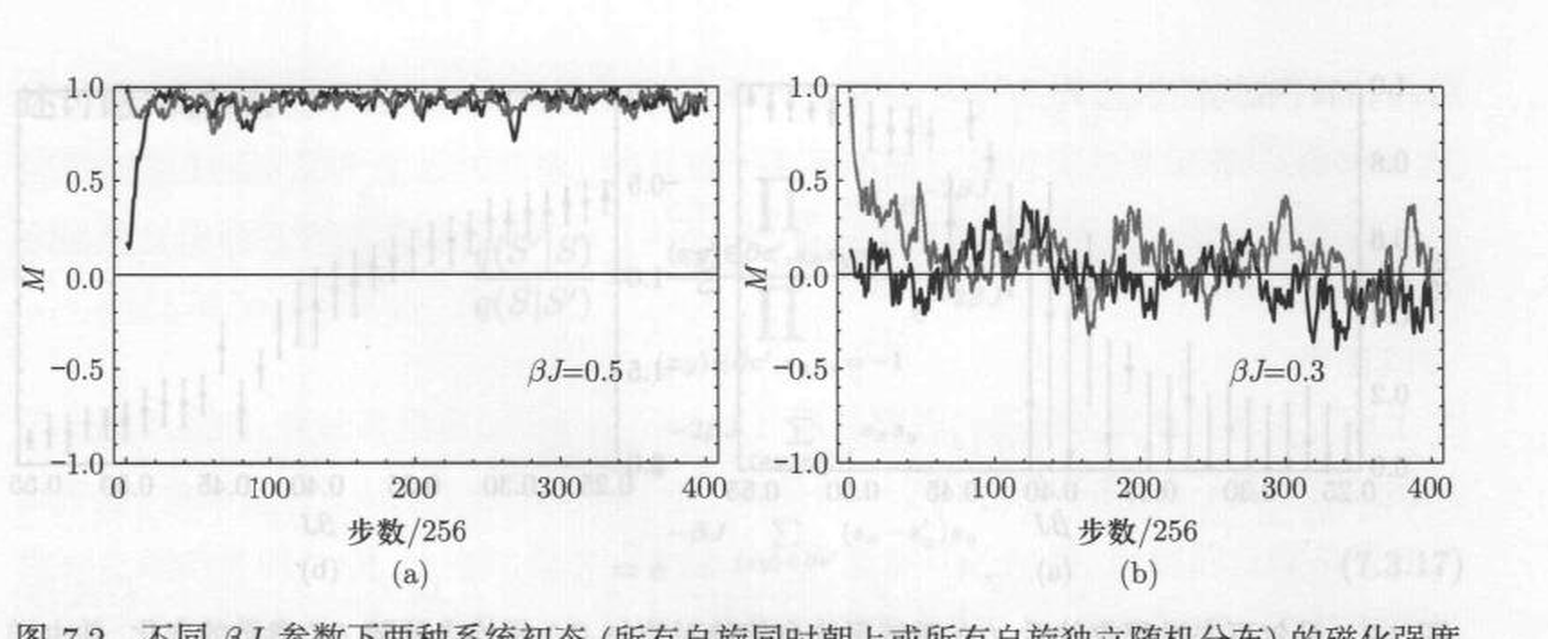
\includegraphics[width=0.96\linewidth]{figures/fig7_2_ising_convergence.png}
\caption{不同 $\beta J$ 参数下两种系统初态（所有自旋同时朝上或所有自旋独立随机分布）的磁化强度随迭代次数的变化}
\label{fig:ising-convergence}
\end{figure}

\begin{algorithmBox}[算法 7.5\quad \rusname{Марков} 过程收敛判据]
\begin{enumerate}[label=\arabic*.,leftmargin=2em]
\item 选取最小迭代次数 $n=4k,\ k\in\mathbb N$。
\item 设后半段的样本已经收敛到所需分布，计算统计量 $x$ 的平均值与方差：
\[
 \langle x\rangle_1=\frac1k\sum_{i=2k+1}^{3k}x_i,\qquad
 \langle x\rangle_2=\frac1k\sum_{i=3k+1}^{4k}x_i,
\]
\[
 \sigma_x^2=\frac1{2k}\sum_{i=2k+1}^{4k}x_i^2
 -\left(\frac1{2k}\sum_{i=2k+1}^{4k}x_i\right)^2.
\]
\item 计算偏差值 $(\langle x\rangle_1-\langle x\rangle_2)^2/\sigma_x^2$，若其小于预设的阈值 $\alpha$，则认为假设成立，结束模拟；否则，令 $k=2k$，继续迭代然后回到第二步。
\end{enumerate}
\end{algorithmBox}

如果假定 \rusname{Марков} 过程最后生成的样本独立同分布，那么偏差量应当大致反比于样本数 $k$。不过由于这些样本通常是强相关的，我们没法对结果做那么强的假定，而只能选取一个较小的常数阈值，例如 $\alpha=0.1$。统计量可以分别取磁化强度和内能，仅当该条件对两个统计量都成立时，我们才认为迭代达到收敛。

利用上述策略，我们计算体系平均自旋的绝对值 $|\mathcal M|$ 和平均内能
\begin{equation}
 U\equiv\frac{\langle\mathcal H\rangle}{L^2}
\tag{7.3.16}
\end{equation}
随 $\beta J$ 的变化。结果如图 7.3 所示，误差棒表示通过样本估算得到的方差。容易发现，方差本身相对平均值就不小，这是因为 $L=16$ 并不大，远远没到热力学极限。其次，数据中有一些明显的离群点，这源自收敛判据在迭代次数还较小的时候就偶然得到了满足。增加 $L$ 或者减小收敛判据中的 $\alpha$ 都能改善结果，但它们同时也会显著增加计算量。而即便对于目前粗糙的计算，单个数据点的最大迭代次数也已经超过了 $10^6$，继续增加计算量显然是难以承受的。因此，我们需要开发新的取样算法。

\originalpage{279}{264}
\begin{figure}[htbp]
\centering
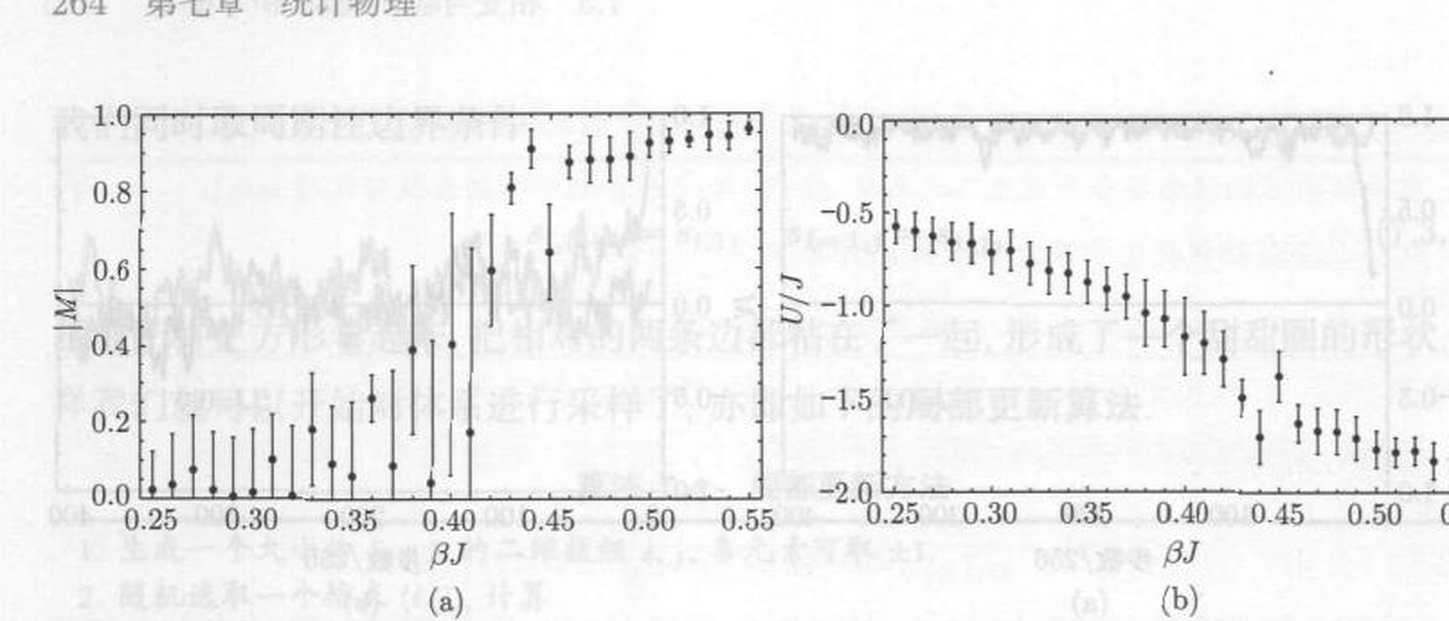
\includegraphics[width=0.94\linewidth]{figures/fig7_3_ising_observables.png}
\caption{\rusname{Марков} 过程收敛后，(a) 系统平均自旋绝对值与 (b) 平均内能随 $\beta J$ 参数的变化，并由样本方差估算得到误差棒}
\label{fig:ising-observables}
\end{figure}

\subsection{Wolff 算法}

1989 年，Wolff 针对类似于 Ising 模型这类在格点上放置磁矩的模型提出了以他命名的采样算法。\footnote{Wolff U. Collective Monte Carlo updating for spin systems. \emph{Phys. Rev. Lett.}, 1989, 62: 361.}

Wolff 算法依旧基于 \rusname{Марков} 过程，但单步迭代的效率远远优于前述的局部更新格式。其核心思想在于，对于一整块自旋方向相同的格点集合，在忽略外场的情况下，将它们整个翻转产生的能量改变仅由其边界决定。而如果想通过一个一个的格点翻转来达到同样的效果，则需要克服其内部相互作用产生的势垒，从而被抑制了。因此，我们需要构造转移概率使得这种集合翻转更容易发生。对于 Ising 模型，算法给出的迭代步骤简述如下。

\begin{algorithmBox}[算法 7.6\quad Wolff 算法]
\begin{enumerate}[label=\arabic*.,leftmargin=2em]
\item 随机取格点 $x$，定义集合 $c=\{x\}$ 和空集 $c'$。
\item 任取 $x\in c$，遍历全部与其相邻且不属于集合 $c$ 和 $c'$ 的元素 $y$，若 $x,y$ 上的自旋同向，则以概率 $1-e^{-2\beta J}$ 将 $y$ 加入集合 $c$，否则不做处理。遍历完成后将 $x$ 从集合 $c$ 移入 $c'$。
\item 重复上一步，直至 $c$ 成为空集。将集合 $c'$ 中全部元素对应格点上的自旋翻转。
\end{enumerate}
\end{algorithmBox}

我们来证明上述过程满足细致平衡条件。如图 7.4 所示，正号代表自旋向上，负号代表自旋向下。将翻转前后系统的状态分别记作 $S$ 和 $S'$。对于 $S\to S'$ 和 $S'\to S$ 这两个互逆的过程，第一步需要选中一个相同的 $x\in c'$，即图中的中点，这对于它们而言概率是相同的。在随后不断扩大集合的过程中，两者的区别体现在 $c'$ 的边界上：对于 $S\to S'$ 是以概率 $e^{-2\beta J}$ 未能将集合外与集合自旋相同的一点纳入集合，即左右两点；对于其逆过程也是以概率 $e^{-2\beta J}$ 未能将集合外与集合自旋相同的一点纳入集合，即上下两点。注意到，两个互逆过程未能纳入集合的点刚好构成了 $c'$ 的完全边界。综合上

\originalpage{280}{265}
述讨论，我们有
\begin{align}
 \frac{q(S'|S)}{q(S|S')}
 &=\frac{\displaystyle\prod_{\langle xy\rangle\in\partial c',\,s_xs_y=1}e^{-2\beta J}}
 {\displaystyle\prod_{\langle xy\rangle\in\partial c',\,s_xs_y=-1}e^{-2\beta J}}
otag\\
 &=e^{-2\beta J\sum_{\langle xy\rangle\in\partial c'}s_xs_y}
otag\\
 &=e^{\beta J\sum_{\langle xy\rangle\in\partial c'}(s_x-s_x')s_y}.
\tag{7.3.17}
\end{align}
这里 $\langle xy\rangle\in\partial c'$ 代表着全部满足 $x\in c',y\notin c'$ 且 $x,y$ 相邻的格点对，表示对集合的边界求和。我们看到，这两个过程发生的概率之比恰好给出了因为集团翻转在边界上所产生的能量差的指数，满足细致平衡条件。

\begin{figure}[htbp]
\centering
\begin{tikzpicture}[scale=0.85]
  \foreach \x/\y/\s in {-1/0/+,0/0/+,1/0/+,0/1/+,0/-1/+,-2/0/+,-1/1/+,1/1/+,2/0/+,1/-1/+,-1/-1/+,0/2/-,2/1/-,2/-1/-,0/-2/-,-2/1/-,-2/-1/-}{
    \node[font=\large] at (\x,\y) {\s};
  }
  \node[below=5pt] at (0,-2.45) {$S$};
  \begin{scope}[xshift=6.5cm]
    \foreach \x/\y/\s in {-1/0/-,0/0/-,1/0/-,0/1/-,0/-1/-,-2/0/+,-1/1/-,1/1/-,2/0/+ ,1/-1/-, -1/-1/-,0/2/+,2/1/+,2/-1/+,0/-2/+,-2/1/+,-2/-1/+}{
      \node[font=\large] at (\x,\y) {\s};
    }
    \node[below=5pt] at (0,-2.45) {$S'$};
  \end{scope}
\end{tikzpicture}
\caption{Wolff 算法细致平衡条件示意图}
\label{fig:wolff-detailed-balance}
\end{figure}

在相变点附近，Wolff 算法的收敛速度相比之前要快得多。我们重复图 7.3 中的计算，但取一个更低的收敛阈值 $\alpha=0.01$，结果如图 7.5 所示。计算中单个数据点使用的迭代次数最大在 $10^4$ 的量级。也就是说，我们减少了两个数量级的计算量，得到的数值结果精度提高了一个数量级。

\begin{figure}[htbp]
\centering
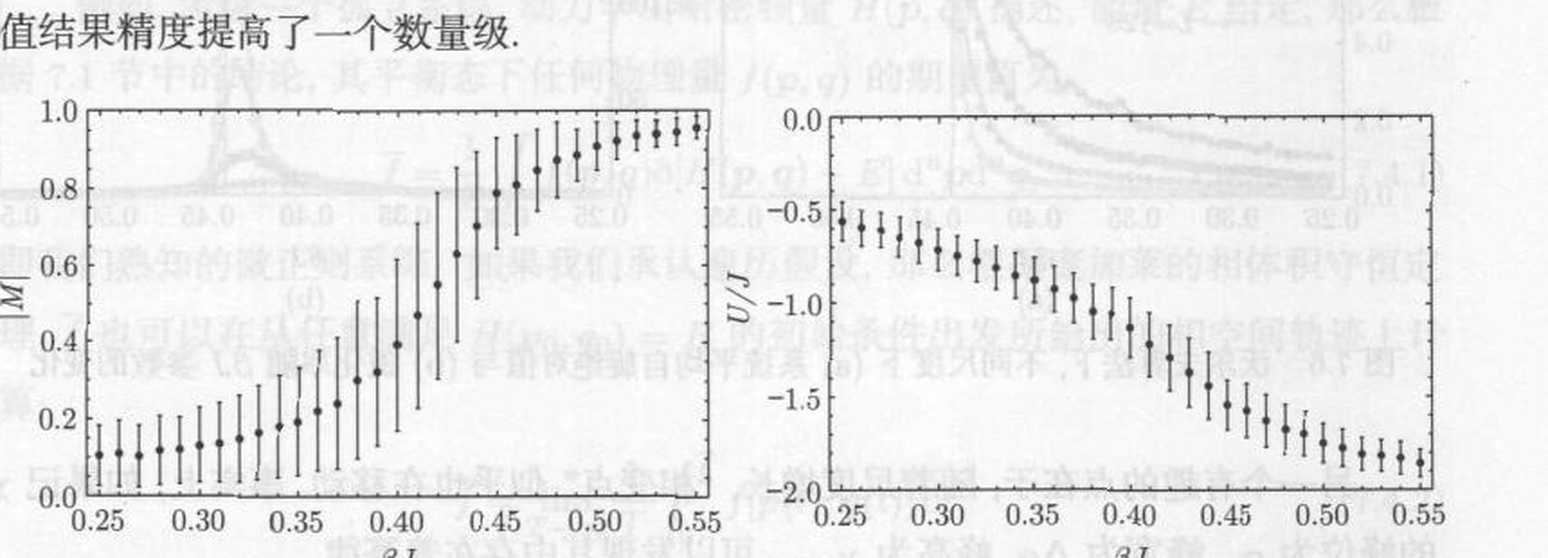
\includegraphics[width=0.94\linewidth]{figures/fig7_5_wolff_observables.png}
\caption{Wolff 算法下，(a) 系统平均自旋绝对值与 (b) 平均内能随 $\beta J$ 参数的变化，并由样本方差估算得到误差棒}
\label{fig:wolff-observables}
\end{figure}

有了如此高效的算法，我们便可以尝试讨论一下热力学极限 $L\to\infty$ 处的行为。在此之前，我们先给出两个热力学量的表达式：热容量

\originalpage{281}{266}
\begin{equation}
\begin{aligned}
 C_H\equiv\left(\frac{\partial U}{\partial T}\right)_H
 &=k_B\beta^2L^2\left\{\frac1Z\sum_S\left(\frac{\mathcal H[S]}{L^2}\right)^2e^{-\beta\mathcal H[S]}-U^2\right\},
\end{aligned}
\tag{7.3.18}
\end{equation}
与磁化率
\begin{equation}
\begin{aligned}
 \chi\equiv\left(\frac{\partial\mathcal M}{\partial H}\right)_T
 &=\beta L^2\left\{\frac1Z\sum_S\left(\frac{\sum_{i,j}s_{i,j}}{L^2}\right)^2e^{-\beta\mathcal H[S]}-\mathcal M^2\right\}.
\end{aligned}
\tag{7.3.19}
\end{equation}
从热力学上讲，这两个量是一阶偏导数的形式，而从统计上来看，它们又各自正比于原始量的方差。对它们的计算是非常直接的。

在图 7.6 中我们分别给出了 $L=16,32,64$ 和 $128$ 的情况下 $|\mathcal M|$ 和 $\chi$ 随 $\beta J$ 变化的关系。可以看到，随着尺度的增长，$|\mathcal M|$ 越来越接近于一个阶跃函数，这预示着热力学极限下相变的发生。此外，$\chi$ 呈现一个单峰函数的形式，峰位与 $|\mathcal M|$ 发生突变的位置重合。这说明在相变发生的位置附近系统的涨落会增强，并且随着尺度的增长，涨落会越来越大。

\begin{figure}[htbp]
\centering
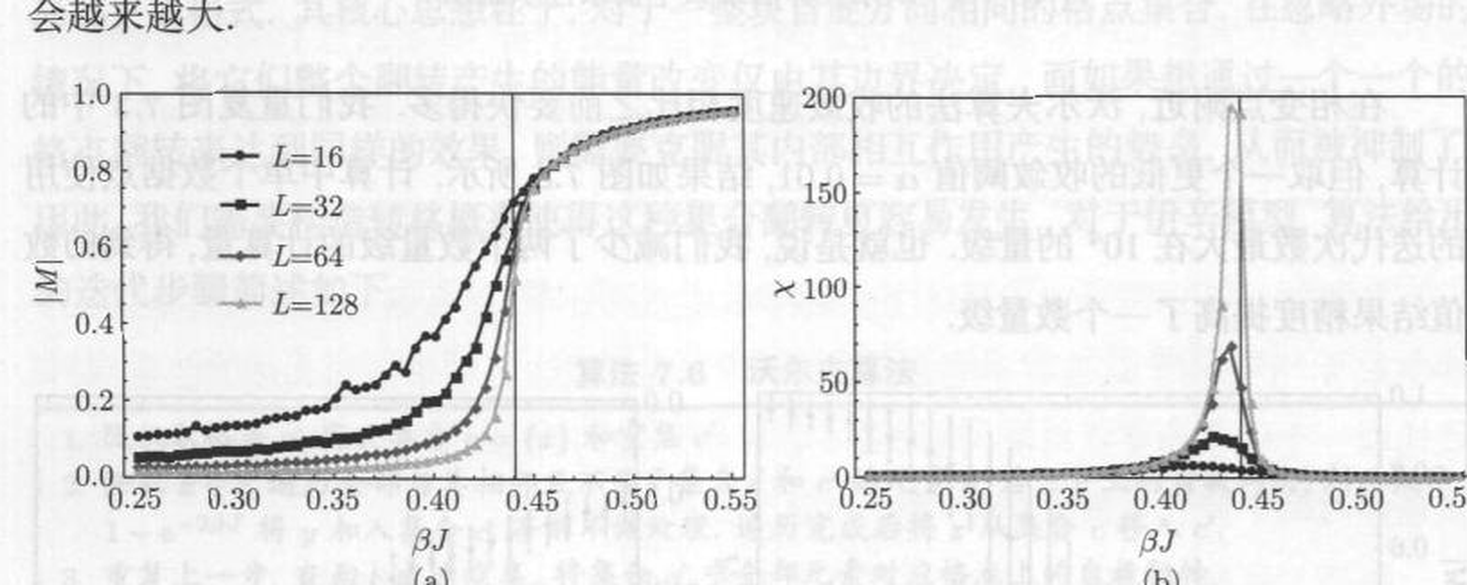
\includegraphics[width=0.94\linewidth]{figures/fig7_6_finite_size.png}
\caption{Wolff 算法下，不同尺度下 (a) 系统平均自旋绝对值与 (b) 磁化率随 $\beta J$ 参数的变化}
\label{fig:ising-finite-size}
\end{figure}

另一个有趣的点在于，随着尺度增长，“相变点”似乎也在移动。事实上，如果记 $\chi$ 的峰位为 $\alpha_c$，峰宽为 $\Delta\alpha$，峰高为 $\chi_{\max}$，可以发现其中存在着幂律
\begin{equation}
 \alpha_c(L)-\alpha_c(\infty)\propto L^{-\nu},\qquad
 \Delta\alpha\propto L^{-\mu},\qquad
 \chi_{\max}\propto L^{\lambda}.
\tag{7.3.20}
\end{equation}
这意味着 Ising 模型在相变点附近存在着某种尺度变换下的自相似性。对于 $U$ 和 $C_H$ 的计算也能给出类似的结论。这是更加普适的临界现象在 Ising 模型上的具体体现，读者可以在统计物理课程中学习到更多相关的内容。

% R22 extends through source scan p.281 / printed p.266.

\originalpage{282}{267}
历史上，人们在使用 Wolff 算法求解一个 $16\times16$ 的 Ising 模型时，发现得到的数值结果依赖于随机数产生器的选取，并且这个差异不能用随机误差来解释。\footnote{Ferrenberg A M, Landau D P, and Wong Y J. Monte Carlo simulations: hidden errors from ``good'' random number generators. \emph{Phys. Rev. Lett.}, 1992, 69: 3382.} 具体而言，在使用反馈移位寄存器 R250
\begin{equation}
X_i=X_{i-103}\oplus X_{i-250}
\tag{7.3.21}
\end{equation}
产生随机数时，在临界温度 $\beta J=\alpha_c(\infty)$ 处计算得到的内能相比准确结果大了数十个标准差，热容量小了上百个标准差。对这个结果的一个简单解释是，由于其生成的随机数列之间的微弱关联，使得在构造一个较大的自旋集团的时候，后面的自旋是否加入依赖于之前的判断，从而使得细致平衡的条件被破坏。事实上，如果使用一个长度更长的反馈移位寄存器 R1279
\begin{equation}
X_i=X_{i-1063}\oplus X_{i-1279},
\tag{7.3.22}
\end{equation}
让关联出现的距离大于最大可能的自旋集团大小 $16\times16=256$，这个奇怪的差异就不会出现。这个结果提醒我们，在使用 Monte Carlo 方法求解一些对随机数独立性有要求的问题时，一定要注意伪随机数对结果是否有影响。

\section{赋予温度：分子动力学热浴}

除去利用 Monte Carlo 过程生成热力学分布外，还存在着一种更“简单粗暴”的办法：直接求解多体的 Hamilton 方程。

例如，考虑一个孤立系统，动力学由 Hamilton 量 $H(p,q)$ 描述，能量 $E$ 给定，那么根据 7.1 节中的结论，其平衡态下任何物理量 $f(p,q)$ 的期望值为
\begin{equation}
\bar f=\frac1Z\int f(p,q)\delta[H(p,q)-E] \,\mathrm d^np\,\mathrm d^nq,
\tag{7.4.1}
\end{equation}
即我们熟知的微正则系综。如果我们承认遍历假设，那么根据庞加莱的相体积守恒定理，$\bar f$ 也可以在从任意满足 $H(p_0,q_0)=E$ 的初始条件出发所给出的相空间轨迹上计算：
\begin{equation}
\bar f=\lim_{T\to\infty}\frac1T\int_0^T f[p(t),q(t)]\,\mathrm dt,
\tag{7.4.2}
\end{equation}
即系综平均等于时间平均。

这样，只要能够稳定求解高维度的常微分方程组，也就是 Hamilton 方程，我们就可以计算微正则系综的任意物理量。这类直接求解的思路被称为分子动力学（molecular dynamics, MD）模拟。而关于 Hamilton 方程的求解，在 2.6 和 4.4 节中已经详细讨论过了。

\originalpage{283}{268}
当然，物理上我们更关心那些可以与外界相互作用、交换能量的正则系综。显然，这是无法直接用 Hamilton 方程来模拟的。通过引入额外的修正项，使得一个系统的时间平均能够近似给出某个指定温度下的正则系综平均，这一过程被称作热浴（thermostat）。本节中我们将讨论其具体实现。而巨正则系综需要考虑粒子数的变化所引起系统自由度的变化，用分子动力学不容易实现，在此不做讨论。

热浴法可以分为几种常见的类型：第一种方法是根据体系平均动能和由温度给出的动能期望的结果差异来对粒子的速度进行改变，包括确定性缩放速度的 Berendsen 方法，随机性缩放速度的 Bussi--Donadio--Parrinello 方法，以及基于粒子随机碰撞和速度重置的 Andersen 方法。第二种方法是基于拓展 Hamilton 量的确定性方法。第三种方法是基于随机微分方程演化的 Langevin 方法。第一种方法的实现方式比较直接，读者可以自行查阅，本节中我们主要讨论后两种方法的实现。

\subsection{确定性方案}

相比于孤立的微正则系综，正则系综可以与外界交换能量，以达到平衡温度。原则上讲，只要我们将系统和外界看作一个整体，那么它应当也能当作微正则系综处理。由能勢修一（Nosé）提出\footnote{Nosé S. A unified formulation of the constant temperature molecular-dynamics methods. \emph{J. Chem. Phys.}, 1984, 81: 511.}并经 Hoover 等人改进得到这样一套方案：通过引入额外的自由度 $(p_s,s)$，扩展相空间的维度，来模拟外界对系统的影响。假设系统原本的 Hamilton 量写作
\begin{equation}
H_0[p,q]=\sum_i\frac{p_i^2}{2m_i}+V(q),
\tag{7.4.3}
\end{equation}
拓展的 Hamilton 量写作
\begin{equation}
H_s[(p,p_s),(q,s)]=\sum_i\frac{p_i^2}{2m_i s^2}+V(q)+\frac{p_s^2}{2Q}+gk_BT\ln s,
\tag{7.4.4}
\end{equation}
对应于 Hamilton 方程
\begin{equation}
\left\{
\begin{aligned}
\dot p_i&=-\frac{\partial V}{\partial q_i},\\
\dot p_s&=\frac1s\left(\sum_i\frac{p_i^2}{m_i s^2}-gk_BT\right),\\
\dot q_i&=\frac{p_i}{m_i s^2},\\
\dot s&=\frac{p_s}{Q}.
\end{aligned}
\right.
\tag{7.4.5}
\end{equation}

\originalpage{284}{269}
这里参数 $g$ 取作 $3N$，为原系统的总自由度，$Q$ 为质量参数，需要根据具体系统来选取。能勢修一--Hoover Hamilton 量中的时间变量 $t$ 不能理解为真实的物理时间 $t'$，它们间存在转换关系 $\mathrm dt'=\mathrm dt/s$。

可以看到，当体系的总动能 $\sum_i p_i^2/(2m_i s^2)$ 小于（大于）能均分定理所给出的 $\frac32Nk_BT$ 时，$\dot p_s$ 为负（正），使得 $s$ 倾向于降低（升高），进而提高（压低）体系的总动能，实现负反馈过程。那么，在长时间平均下，可以预见体系的总动能将在 $\frac32Nk_BT$ 附近振荡，各种物理量的时间平均也更接近于正则系综的结果。

在能勢修一--Hoover 方法中，负反馈的引入基于直觉，缺乏严格的证明来保证其有效性。事实上，即便是最简单的谐振子系统，该方法也不能给出一个正确的正则分布。\footnote{Posch H A, Hoover W G, and Vesely F J. Canonical dynamics of the Nosé oscillator: stability, order, and chaos. \emph{Phys. Rev. A}, 1986, 33: 4253.} 为此，人们从能勢修一--Hoover 方法出发进一步推广得到了能勢修一--Hoover 链方法。\footnote{Martyna G J, Klein M L, and Tuckerman M. Nosé--Hoover chains: the canonical ensemble via continuous dynamics. \emph{J. Chem. Phys.}, 1992, 97: 2635.} 它在原本的额外自由度 $s$ 的基础上又引入若干新的自由度，用变量 $s_1,s_2,\ldots,s_N$ 表示，其中每个自由度只与其相邻的变量耦合，于是可以得到一串包含变量 $s_1,s_2,\ldots,s_N$ 及其动量的拓展的微分方程组。实践表明，一般情况下能勢修一--Hoover 链只需要取到长度为 4 或 5，就可以很好地用扩展系统的微正则系综分布来模拟原始体系的正则系综分布。

如何让一个经典或量子系统从确定的状态演化到热力学分布，这是一个深刻的物理问题，目前也属于热门的研究领域之一。

\subsection{随机微分方程}

另一类用以模拟外界对系统作用的热浴方案是，将外界的驱动看作一个随机的分布。其来源于对 Brown 运动的研究，以及为其所发展出来的 Langevin 方程。Brown 运动是一个演示热浴的好例子：花粉颗粒本身是一个确定性的系统，但由于浸泡在一定温度的水（外界）中，会受到水分子热运动所引起的不断碰撞（相互作用），最后达到热平衡态。

Brown 运动可以用 Langevin 方程描述：
\begin{equation}
m\ddot x=-\gamma\dot x+f(t),
\tag{7.4.6}
\end{equation}
等式右端两项分别为黏滞阻力和随机相互作用力。直接计算便可以证明，如果随机相互作用力满足
\begin{equation}
\overline{f(t)f(t')}=2\gamma k_BT\delta(t-t'),
\tag{7.4.7}
\end{equation}

\originalpage{285}{270}
那么体系的速度关联函数为
\begin{equation}
\overline{\dot x(t)\dot x(t')}=\frac{k_BT}{m}e^{-|t-t'|\gamma/m}.
\tag{7.4.8}
\end{equation}
取 $t=t'$ 我们便重新得到了能均分定理。注意到随机项的自关联函数正比于黏滞阻力系数，这个结果被称为 Einstein 关系。

将上述方程应用到分子动力学中就可以得到 Langevin 热浴法，也就是在运动方程的动量演化方程中加入两个额外的力
\begin{equation}
\left\{
\begin{aligned}
\dot q_i&=\frac{p_i}{m_i},\\
\dot p_i&=-\frac{\partial V}{\partial q_i}-\gamma_i p_i+f_i.
\end{aligned}
\right.
\tag{7.4.9}
\end{equation}
在数值求解时，通常会将每一时刻的 $f_i$ 取作中心为零的 Gauß 分布，其方差为 $\sigma_i^2=2\gamma_i k_BT/\Delta t$，$\Delta t$ 是分子动力学模拟的积分时间步长。对这类随机函数更精细的描述可以通过 Gauß 过程来实现。

Brown 运动的研究对统计物理的建立起到了重要的推动作用，同时该工作也推进了应用数学中随机微积分的研究。Langevin 动力学只是随机动力学的一个特殊例子，随机过程和动力学在很多其他科学和工程研究中也具有广泛的意义。关于随机微分方程的更详细的介绍远远超出了本书的范畴，感兴趣的读者可以查阅更加专业的资料。值得一提的是，Langevin 动力学等随机过程在处理复杂的函数优化问题时也可以起到重要的作用。在下一章中介绍更加复杂的机器学习模型的参数优化时，也会提到基于随机性的优化算法所带来的帮助。

\section{非平衡过程：粒子网格法}

在前面几节中，我们见识到了求解一个热力学系统的平衡态是多么困难：即使是一个简单的二维 Ising 模型，尺度一大算起来也不容易。问题的关键是关联：体系中的不同粒子之间相互影响，让体系的自由度呈指数增长，以至于无法处理。

Boltzmann 在讨论稀薄气体时遇见了同样的问题，他决定转过头去研究单粒子分布的演化，从而给出了他的方程
\begin{equation}
\partial_t f+\mathbf v\cdot\nabla_{\mathbf r}f+\mathbf F\cdot\nabla_{\mathbf p}f=f_{\text{碰撞}}.
\tag{7.5.1}
\end{equation}
注意这里包含了对时间的偏导数，从而研究对象是一个处在非平衡态的系统。方程左端的后两项分别代表粒子因运动和受外场作用而导致分布函数在实空间和动量空间上的漂移，方程右端则是碰撞项，可以形式地写作
\begin{equation}
f_{\text{碰撞}}(\mathbf r,\mathbf p)=\int K f(\mathbf r,\mathbf p;\mathbf p_1;\mathbf p'_1,\mathbf p'_2;t)\delta(\mathbf p+\mathbf p_1-\mathbf p'_1-\mathbf p'_2)\,\mathrm d^3p'_1\,\mathrm d^3p'_2\,\mathrm d^3p_1.
\tag{7.5.2}
\end{equation}

\originalpage{286}{271}
其中 $K$ 代表弹性碰撞过程 $\mathbf p'_1\mathbf p'_2\to \mathbf p\mathbf p_2$ 发生的概率，对应着碰撞截面，通常可以写成相对动量
\begin{equation}
g=|\mathbf p-\mathbf p_2|=|\mathbf p'_1-\mathbf p'_2|
\tag{7.5.3}
\end{equation}
和散射角
\begin{equation}
\theta=\arccos\!\left[(\mathbf p-\mathbf p_2)\cdot(\mathbf p'_1-\mathbf p'_2)/g^2\right]
\tag{7.5.4}
\end{equation}
的函数。

我们看到，为了求解单粒子分布的演化，必须知道双粒子联合分布。同样，我们可以写下 $n$ 粒子分布所满足的方程，其中的碰撞项一定包含 $n+1$ 粒子的联合分布。这样，求解起来就无穷无尽了。为了解决这个问题，Boltzmann 做出了著名的分子混沌性假设：两体分布函数可以近似拆分成单体分布函数的乘积：
\begin{equation}
f(\mathbf r_1,\mathbf p_1;\mathbf r_2,\mathbf p_2;t)=f(\mathbf r_1,\mathbf p_1;t)f(\mathbf r_2,\mathbf p_2;t).
\tag{7.5.5}
\end{equation}
在这个假设成立的基础上，只需要求解六维相空间中的分布函数，我们就能得到系统的平衡态。在引入分子混沌性假设将两体分布函数写成两个单体分布函数的乘积后，Boltzmann 方程成了一个非线性积分微分方程。这个非线性与求解量子多体问题的 HF 方法中的非线性的来源是类似的，都源自将多自由度函数近似写成单自由度函数的某种组合。它们都是更一般性的平均场方法的特殊情况。

尽管 Boltzmann 方程的维度相比最初的 $6n$ 维已经大大降低，但直接求解仍旧是几乎不可能的事情。此外，Boltzmann 方程假定了粒子之间的相互作用都是短程力，仅当两个粒子空间位置重合时才会存在相互作用。然而，如果我们考察粒子带电荷的情形，电磁作用作为长程力无法用碰撞来近似，我们就必须求解与 Maxwell 方程组相耦合的 \rusname{Власов}（Vlasov）方程
\begin{equation}
\left\{
\begin{aligned}
\partial_t f_s+\mathbf v_s\cdot\nabla_{\mathbf r}f_s+q_s(\mathbf E+\mathbf v_s\times\mathbf B)\cdot\nabla_{\mathbf p}f_s&=0,\\
\mathbf v_s&=\frac{\mathbf p c}{\sqrt{m_s^2c^2+p^2}},\\
\rho(\mathbf r,t)&=\sum_s N_s q_s\int f_s(\mathbf r,\mathbf p,t)\,\mathrm d^3p,\\
\mathbf J(\mathbf r,t)&=\sum_s N_s q_s\int \mathbf v_s f_s(\mathbf r,\mathbf p,t)\,\mathrm d^3p.
\end{aligned}
\right.
\tag{7.5.6}
\end{equation}
此处我们假设了系统由多种不同组分的粒子构成，用指标 $s$ 标记，每类粒子有 $N_s$ 个，具有电荷 $q_s$ 与质量 $m_s$。速度--动量关系使用了相对论性的表达式，这是因为 \rusname{Власов} 方程常用于描述极端相对论性等离子体的动力学。粒子间的相互作用通过电磁场传播：由电荷与电流密度产生电磁场，再由电磁场作用于粒子的分布。

\originalpage{287}{272}
虽然由于去掉了碰撞项，该方程是一个纯粹的微分方程，但是更多的自由度被非线性地耦合了进来，求解起来也不比 Boltzmann 方程容易。

此时我们再次将目光投向了 Monte Carlo 方法：既然求解的是分布函数随时间的演化，我们能否直接按照初始时刻的分布函数撒一批样本，然后根据各个时刻样本的情况估算分布函数，进而决定样本随时间的演化呢？本节中我们便将以一维 \rusname{Власов} 方程为例，演示这种方法的具体实现。

\subsection{\rusname{Власов} 方程}

首先假定我们根据 $t=t_0$ 时刻的分布 $f_s(\mathbf r,\mathbf p,t_0)$ 生成了一系列样本 $(\mathbf r_{ks},\mathbf p_{ks})$，每类粒子的样本数为 $Q_s$。它们在电磁场中的演化满足方程
\begin{equation}
\left\{
\begin{aligned}
\dot{\mathbf p}_{ks}&=q_s[\mathbf E(\mathbf r,t)+\dot{\mathbf r}_{ks}\times\mathbf B(\mathbf r,t)],\\
\dot{\mathbf r}_{ks}&=\frac{\mathbf p_{ks}c}{\sqrt{m_s^2c^2+p_{ks}^2}}.
\end{aligned}
\right.
\tag{7.5.7}
\end{equation}
第一个问题是如何根据 $t$ 时刻的样本来估计分布函数。注意到电磁场是由电荷密度和电流密度分布决定的，我们可以不去管动量空间的分布。最简单的策略自然是使用 $\delta$ 函数：
\begin{equation}
\rho(\mathbf r)=\sum_s q_s\frac{N_s}{Q_s}\sum_k\delta(\mathbf r-\mathbf r_{ks}).
\tag{7.5.8}
\end{equation}
不过这种无穷大的东西在数值上通常不好处理。另一种策略是将空间划分成网格，然后使用分段线性函数。对于一维问题，我们以间隔 $h$ 等距地取格点 $\{x_i\}$，可以按下式估计得到电荷密度：
\begin{equation}
\rho(x_i)=\sum_s q_s\frac{N_s}{Q_s}\left(\sum_{x_{i-1}<r_{ks}<x_i}\frac{r_{ks}-x_{i-1}}{h^2}+\sum_{x_i<r_{ks}<x_{i+1}}\frac{x_{i+1}-r_{ks}}{h^2}\right).
\tag{7.5.9}
\end{equation}
电流密度的计算也是类似的：
\begin{equation}
J(x_i)=\sum_s q_s\frac{N_s}{Q_s}\left(\sum_{x_{i-1}<r_{ks}<x_i}\frac{r_{ks}-x_{i-1}}{h^2}v_{ks}+\sum_{x_i<r_{ks}<x_{i+1}}\frac{x_{i+1}-r_{ks}}{h^2}v_{ks}\right).
\tag{7.5.10}
\end{equation}
有了电流与电荷分布，我们来考虑如何求解电磁场的演化。当限定电磁场仅依赖于时间 $t$ 和一维坐标 $x$ 时，电磁场可以拆分成互不影响的横向分量和纵向分量，纵向分量有显式的表达式
\begin{equation}
\left\{
\begin{aligned}
E_x&=-\frac1{\epsilon_0}\int \rho\,\mathrm dx=-\frac1{\epsilon_0}\int J_x\,\mathrm dt,\\
B_x&=C.
\end{aligned}
\right.
\tag{7.5.11}
\end{equation}

\originalpage{288}{273}
而横向分量满足方程
\begin{equation}
\left\{
\begin{aligned}
\partial_t B_z&=-\partial_x E_y,\\
\partial_t B_y&=\partial_x E_z,\\
\partial_t E_z&=c^2\partial_x B_y-\frac1{\epsilon_0}J_z,\\
\partial_t E_y&=-c^2\partial_x B_z-\frac1{\epsilon_0}J_y,
\end{aligned}
\right.
\tag{7.5.12}
\end{equation}
为一个四分量的偏微分方程。注意到电场与磁场之间对偶的形式，我们可以借助蛙跳法的思想，构造交错网格来离散化上述方程。

具体而言，我们已知电流密度 $J$ 在空间网格 $\{x_i\}$ 和时间网格 $\{t_j\}$ 上的分布 $J^{i,j}$，而它所在的方程又对应有电场的时间偏导数和磁场的空间偏导数，那么我们将电场和磁场的网格分别在时间和空间上错开半步，应用中心差分
\begin{equation}
\left\{
\begin{aligned}
\frac{E_z^{i,j+1/2}-E_z^{i,j-1/2}}{\Delta t}&=c^2\frac{B_y^{i+1/2,j}-B_y^{i-1/2,j}}h-\frac1{\epsilon_0}J_z^{i,j},\\
\frac{E_y^{i,j+1/2}-E_y^{i,j-1/2}}{\Delta t}&=-c^2\frac{B_z^{i+1/2,j}-B_z^{i-1/2,j}}h-\frac1{\epsilon_0}J_y^{i,j}.
\end{aligned}
\right.
\tag{7.5.13}
\end{equation}
借助这个差分格式，在已知 $t_j$ 时刻的电流密度和磁场分布，以及 $t_{j-1/2}$ 时刻的电场分布的情况下，我们可以求得 $t_{j+1/2}$ 时刻的电场分布。

随后我们可以用类似的办法处理前两个方程：
\begin{equation}
\left\{
\begin{aligned}
\frac{B_z^{i+1/2,j+1}-B_z^{i+1/2,j}}{\Delta t}&=-\frac{E_y^{i+1,j+1/2}-E_y^{i,j+1/2}}h,\\
\frac{B_y^{i+1/2,j+1}-B_y^{i+1/2,j}}{\Delta t}&=\frac{E_z^{i+1,j+1/2}-E_z^{i,j+1/2}}h.
\end{aligned}
\right.
\tag{7.5.14}
\end{equation}
这样，借助之前获得的信息，我们可以进一步求解 $t_{j+1}$ 时刻的磁场分布。

下一步便是计算粒子的运动了，注意到我们需要的是 $t_{j+1}$ 时刻的空间坐标
\begin{equation}
\frac{r_{ks}^{j+1}-r_{ks}^{j}}{\Delta t}=\mathbf e_x\cdot\frac{\mathbf p_{ks}^{j+1/2}c}{\sqrt{m_s^2c^2+|\mathbf p_{ks}^{j+1/2}|^2}},
\tag{7.5.15}
\end{equation}
为此要求解的是 $t_{j+1/2}$ 时刻的运动方程
\begin{equation}
\frac{\mathbf p_{ks}^{j+1/2}-\mathbf p_{ks}^{j-1/2}}{\Delta t}=q_s\left[\mathbf E(r_{ks}^{j},t_j)+\frac{\mathbf v_{ks}^{j+1/2}+\mathbf v_{ks}^{j-1/2}}2\times\mathbf B(r_{ks}^{j},t_j)\right],
\tag{7.5.16}
\end{equation}
故我们需要计算任意空间坐标上的电磁场，这可以通过分段线性插值处理：
\begin{equation}
\left\{
\begin{aligned}
\mathbf E(r,t_j)&=\frac{r-x_i}{h}\frac{\mathbf E^{i+1,j+1/2}+\mathbf E^{i+1,j-1/2}}2+\frac{x_{i+1}-r}{h}\frac{\mathbf E^{i,j+1/2}+\mathbf E^{i,j-1/2}}2,
\quad x_i\le r<x_{i+1},\\
\mathbf B(r,t_j)&=\frac{r-x_{i-1/2}}h\mathbf B^{i+1/2,j}+\frac{x_{i+1/2}-r}h\mathbf B^{i-1/2,j},
\quad x_{i-1/2}\le r<x_{i+1/2}.
\end{aligned}
\right.
\tag{7.5.17}
\end{equation}

\originalpage{289}{274}
在给出电磁场后，由于相对论性速度--动量关系和磁场项，式 (7.5.16) 是一个非线性的自治迭代格式，通常简单做数步迭代就能得到较好的结果。

到目前为止，我们已经拥有了进行完整计算所需要的全部步骤了，迭代求解过程总结如下：
\begin{algorithmBox}[算法 7.7\quad 交错网格法]
\begin{enumerate}[label=\arabic*.,leftmargin=2em]
\item 根据式 (7.5.10)，利用 $t_j$ 时刻的样本分布计算此时网格上的电流密度 $J^{i,j}$。
\item 根据式 (7.5.13)，利用 $t_j$ 时刻的电流密度 $J^{i,j}$ 和磁场分布 $B^{i+1/2,j}$ 将电场分布从 $t_{j-1/2}$ 更新至 $t_{j+1/2}$ 时刻。
\item 根据式 (7.5.14)，利用 $t_{j+1/2}$ 时刻的电场分布将磁场分布更新至 $t_{j+1}$ 时刻。
\item 对于每一个粒子，根据式 (7.5.17) 内插得到 $t_j$ 时刻其所在位置的电磁场强度。
\item 求解自治方程 (7.5.16) 式，将每个粒子的动量更新至 $t_{j+1/2}$ 时刻。
\item 根据式 (7.5.15)，将粒子坐标更新至 $t_{j+1}$ 时刻。
\end{enumerate}
\end{algorithmBox}

再添加上恰当的边界条件和初始条件，我们就可以尝试求解实际问题了。

这类同时求解粒子群的常微分方程以及格点上的偏微分方程的算法被称为粒子网格法（particle in cell, PIC），在等离子体物理中有着广泛的应用。将电磁场换作压强场、密度场，这类算法也能应用于求解流体力学中的部分问题。

\subsection{Bohm 力学}

上述方法还有一个意想不到的应用：求解 Bohm 导航波诠释下的 Schrödinger 方程。让我们考虑单粒子定态 Schrödinger 方程
\begin{equation}
E\psi=-\frac1{2m}\nabla^2\psi+V\psi.
\tag{7.5.18}
\end{equation}
将波函数写成振幅和相位分解的形式 $\psi=R\exp(iS)$，代回上式，得到两个实方程
\begin{equation}
\left\{
\begin{aligned}
\partial_tR+\frac1{2m}(R\nabla^2S+2\nabla R\cdot\nabla S)&=0,\\
\partial_tS+\frac1{2m}|\nabla S|^2+V-\frac1{2m}\frac{\nabla^2R}{R}&=0.
\end{aligned}
\right.
\tag{7.5.19}
\end{equation}
引入 $\rho=R^2$，第一个方程可以进一步改写成概率流守恒的形式
\begin{equation}
\partial_t\rho+\nabla\cdot\left(\rho\frac{\nabla S}{m}\right)=0,
\tag{7.5.20}
\end{equation}
只要将 $\nabla S/m$ 看作粒子的速度，这个方程就可以理解成概率密度分布 $\rho$ 的守恒方程。而第二个方程又非常类似于经典 Hamilton--Jacobi 方程，只不过多了一项
\begin{equation}
Q=-\frac1{2m}\frac{\nabla^2R}{R},
\tag{7.5.21}
\end{equation}
这一项被称作量子势。

\originalpage{290}{275}
那么，我们可以将波函数理解成大量相同经典粒子的集合，这些粒子在外势场 $V$ 下运动，并通过量子势 $Q$ 相互作用。量子势与粒子数密度的绝对大小无关，这让它同寻常的相互作用大不相同。不过，在使用 Monte Carlo 方法进行数值模拟上，过程完全是类似的：先根据 $t=t_0$ 时刻的波函数生成初始粒子样本 $\{(r_k,p_k)\}$，然后开始迭代：
\begin{enumerate}[label=(\arabic*),leftmargin=2em]
\item 根据全部粒子的坐标估计格点上的概率密度分布 $\rho$；
\item 通过二阶差分计算格点上的量子势 $Q$ 以及作用力 $\mathbf F=-\nabla(V+Q)$；
\item 对全部粒子，通过内插计算其所处位置的作用力，并使用蛙跳法更新动量与位置：
\[
p_k(t_{i+1/2})=p_k(t_{i-1/2})+\mathbf F(r_k,t_i)\Delta t,
\]
\[
r_k(t_{i+1})=r_k(t_i)+p_k(t_{i+1/2})\Delta t.
\]
\end{enumerate}
显然，这个计算过程要比直接求解单粒子 Schrödinger 方程复杂多了。因此，除了少数物理图像诠释上的目的，人们几乎不会使用 Bohm 的这一套理论。

\section{量子多体系统：量子蒙特卡洛}

在本章的前几节中，我们讨论了如何利用 Monte Carlo 方法处理统计物理中的各种问题，它们都属于经典物理的范畴。由于 Monte Carlo 方法复杂度几乎与问题维度无关的特性，它在这些问题上都显示了相较于其他方法的优势。而量子力学中的多体系统也是一个典型的高维问题，我们自然期待 Monte Carlo 方法在这一问题上面有所发挥。

\subsection{能量期望值}

一个直截了当的问题便是计算 Hamilton 算符的期望值
\begin{equation}
E=\langle\Psi|H|\Psi\rangle.
\tag{7.6.1}
\end{equation}
对于一次量子化的情形，波函数可以写作全部粒子坐标 $R:\{r_1,\ldots,r_N\}$ 的函数 $\Psi(R)=\langle R|\Psi\rangle$，那么有
\begin{equation}
E=\int \Psi^*(R)\hat H\Psi(R)\,\mathrm dR=\int |\Psi(R)|^2\frac{\hat H\Psi(R)}{\Psi(R)}\,\mathrm dR,
\tag{7.6.2}
\end{equation}
是一个高维积分。注意到波函数的模方 $|\Psi(R)|^2$ 是一个正定归一的分布函数，那么我们便可以借助 Monte Carlo 积分的思想，根据分布 $|\Psi(R)|^2$ 生成样本 $R_i$，给出能量的表达式
\begin{equation}
E=\lim_{N\to\infty}\frac1N\sum_{i=1}^{N}E_{\mathrm{loc}}(R_i),
\tag{7.6.3}
\end{equation}

\originalpage{291}{276}
其中 $E_{\mathrm{loc}}\equiv \hat H\Psi(R_i)/\Psi(R_i)$ 一般称为局域能量。

在上述计算过程中，最关键的步骤是给定波函数以后对于粒子空间位置的采样。在采样中，体系的“量子性”并不会起到任何作用，只需要与经典粒子一样采用 Monte Carlo 链的思想，通过含选过程的随机游走即可实现。

\subsection{随机游走}

量子 Monte Carlo 中常用 Metropolis--Hastings 抽样方法。与 7.3 节中介绍过的 Barker 算法一样，这也是一种基于含选法和复合抽样法的方案。

\begin{algorithmBox}[算法 7.8\quad Metropolis--Hastings 算法]
\begin{enumerate}[label=\arabic*.,leftmargin=2em]
\item 对于系统的可能状态 $x,y$，定义移动概率 $t(y|x)$ 和接受概率 $a(y|x)$，满足
\[
\int t(y|x)\,\mathrm dy=1,\qquad a(y|x)=\min\left\{1,\frac{P(y)t(x|y)}{P(x)t(y|x)}\right\}.
\]
\item 从状态 $x$ 出发，以分布 $t(z|x)$ 给出抽样 $z$。
\item 以概率 $a(z|x)$ 选择 $y=z$，以概率 $1-a(z|x)$ 选择 $y=x$。
\end{enumerate}
\end{algorithmBox}

可以验证，这样得到的条件概率 $q(y|x)=a(y|x)t(y|x)$ 满足细致平衡条件 $q(y|x)P(x)=q(x|y)P(y)$，可以使得其演化得到的分布满足 $P(x)$。

对于本节中的问题，试探移动的一个自然选择是（$\Delta$ 为一参数，用以控制进行试探移动）
\begin{equation}
t(y|x)=
\begin{cases}
1/\Delta,&|y-x|<\Delta/2,\\
0,&\text{其他情况}.
\end{cases}
\tag{7.6.4}
\end{equation}
其中对于多粒子体系，状态 $x,y:\{r_1,\ldots,r_N\}$，该试探移动意味着将粒子坐标沿着各个方向按照均匀分布进行一个小的随机移动。具体操作过程中还可以进一步细分一些具体的技巧，比如每次移动所有粒子或者每次只移动一个粒子，关于这些具体的操作这里不展开讨论。

\subsection{变分计算}

然而，物理上大家更关心的问题是，如何对于给定的 Hamilton 量，求得其对应的基态波函数。为此，我们将 5.4 节中采用的思路做推广：对于某个问题，可以预先假定一个波函数的形式 $\Psi_\theta(R)$，其中 $\theta$ 是一些待定参数。由于 Hamilton 算符是有下界的，那么任意波函数的能量期望值总是大于等于基态能量：
\begin{equation}
E_\theta=\int \Psi_\theta^*(R)\hat H\Psi_\theta(R)\,\mathrm dR\ge E_0,
\tag{7.6.5}
\end{equation}

\originalpage{292}{277}
当且仅当其波函数为基态波函数时取等。原则上讲，只要求得 $E_\theta$ 的极小值位置，我们便获得了体系基态波函数一个不错的近似。

当然，$\Psi_\theta(R)$ 的形式对于最后结果的准确性是很重要的，我们称之为波函数拟设（ansatz）。只当波函数拟设能够充分地表达可能的多体波函数时，变分 Monte Carlo 才可以得到真正的基态，否则它给出的只是该拟设极限下的基态。

拟设是决定变分 Monte Carlo 精度的关键因素，一个复杂的量子多体体系，其拟设也是复杂且未知的。从提高计算精度的角度出发，我们主要的目标就是提高拟设的表达能力，从而让它能够在变分优化过程中更加逼近真实的基态。从探究物理本质的角度出发，找出拟设形式背后对应的物理意义能够让我们对量子多体物理有更加清楚的理论认识。同时，它也可以让我们在有限的计算能力下更好地描述某个特殊的量子多体态。在拟设的设计中也有一些特殊的技术问题。比如，当我们考虑开边界的有限体系和固体这样的周期性体系时，拟设需要相应的设计。再比如，拟设的构造有时候也需要考虑一些波函数需要满足的尖点（cusp）条件（如 6.4.2 小节中所讨论的），从而在 Monte Carlo 采样中减弱某些发散项带来的大的涨落。

\subsection{优化算法}

$E_\theta$ 的极小化问题可以借助近似的 Newton 法来处理。写下 $E_{\theta+\phi}$ 在 $\theta$ 处的二阶 Taylor 展开
\begin{equation}
E_{\theta+\phi}\approx E_\theta+\phi^{\mathrm T}\nabla_\theta E_\theta+\frac12\phi^{\mathrm T}\mathbf M\phi,
\tag{7.6.6}
\end{equation}
其中梯度算符给出
\begin{equation}
\begin{aligned}
(\nabla_\theta E_\theta)_i
&=\langle\Psi|H|\Phi_i\rangle+(\partial_{\theta_i}\langle\Psi|)H|\Psi\rangle\\
&=\langle\Psi|H|\Phi_i\rangle+\langle\Phi_i|H|\Psi\rangle,
\end{aligned}
\tag{7.6.7}
\end{equation}
我们引入了记号 $|\Phi_i\rangle\equiv\partial_{\theta_i}|\Psi\rangle$。而 Hessian 矩阵为
\begin{equation}
\begin{aligned}
(\mathbf M)_{ij}={}&\langle\Phi_i|H|\Phi_j\rangle+\langle\Phi_j|H|\Phi_i\rangle\\
&+\langle\Psi|H|\partial_{\theta_i}\partial_{\theta_j}\Psi\rangle+(\partial_{\theta_i}\partial_{\theta_j}\langle\Psi|)H|\Psi\rangle.
\end{aligned}
\tag{7.6.8}
\end{equation}
为了计算方便，作为一个近似，我们忽略上式的第二行，也就是波函数对参数的二阶导数，那么 $E_\theta$ 的二阶导数都可以用 $H$ 在 $|\Psi\rangle$ 和 $|\Phi_i\rangle$ 下的交叠矩阵元给出，而这些矩阵元又都可以通过相同的 Monte Carlo 方法来计算。这样，我们便可以给出优化迭代的下一步：
\begin{equation}
\theta+\phi=\theta-\mathbf M^{-1}\nabla_\theta E_\theta.
\tag{7.6.9}
\end{equation}

\originalpage{293}{278}
显然，由于在计算二阶导数时做了近似，这个迭代不具有真正 Newton 迭代的二阶收敛特性。但考虑到二阶导数的严格计算将增大不少计算量，而 Monte Carlo 方法得到的矩阵元素本身也存在误差，这个近似还是能够接受的。

有时候，人们在做波函数拟设的时候不会将其归一化，或者归一化在解析上非常困难，此时会将波函数的归一化系数也当作待定参数，并求解带归一化约束的极值问题。

另一种更粗略，但单次计算量更低的算法称为随机重组（stochastic reconfiguration）算法。其思想基于 6.2 节中提到过的虚时演化：在选取迭代步时，我们希望有如下关系近似成立：
\begin{equation}
|\Psi_{\theta+\phi}\rangle\approx e^{-\tau H}|\Psi_\theta\rangle\approx (I-\tau H)|\Psi_\theta\rangle.
\tag{7.6.10}
\end{equation}
如果 Hamilton 量 $H$ 的本征谱同时存在上下界，\footnote{不过，对于带有动能项的连续系统来说，其本征谱是没有上界的。} 并满足 $|1-E_{\min}\tau|>|1-E_{\max}\tau|$ 以及 $E_{\min}<0$，那么 $1-E_{\min}\tau$ 将是算符 $I-\tau H$ 模最大的本征值，根据幂法的原理，反复迭代将使波函数向其所对应的本征向量逼近。而若不将指数算符做展开，这相当于求解基态的虚时传播方法。

随后便是考虑如何选取 $\phi$ 使上述迭代式近似成立。将 $|\Psi_{\theta+\phi}\rangle$ 展开到一阶，有
\begin{equation}
\sum_i\phi_i|\Phi_i\rangle\approx-\tau H|\Psi\rangle.
\tag{7.6.11}
\end{equation}
在最小二乘的意义下，这相当于要求线性代数方程组
\begin{equation}
\sum_i\langle\Phi_j|\Phi_i\rangle\phi_i=-\tau\langle\Phi_j|H|\Psi\rangle
\tag{7.6.12}
\end{equation}
成立，计算上式中的矩阵元并求解线性代数方程组便可得到优化的下一个迭代步。相比近似的 Newton 法，这个算法省去了不同 $|\Phi_i\rangle$ 之间的 Hamilton 矩阵元的计算，单步效率更高，对于那些拟设参数空间维度相当高的问题而言具有不小优势。

\subsection{实际计算：液氦}

1965 年，McMillan 第一次采用变分 Monte Carlo 方法对液态 $^4$He 体系进行了计算。\footnote{McMillan W L. Ground state of liquid He$^4$. \emph{Phys. Rev.}, 1965, 138: A442.} 他略去了 $^4$He 的内部激发，并认为 $^4$He 原子之间的相互作用可以由 Lennard--Jones 势 $V(r)=4\epsilon[(\sigma/r)^{12}-(\sigma/r)^6]$ 给出。那么，可以写下液氦的 Hamilton 量
\begin{equation}
\hat H=-\sum_i\frac{\nabla_i^2}{2m}+\sum_{i<j}V(r_{ij}).
\tag{7.6.13}
\end{equation}

\originalpage{294}{279}
对于该体系，可以采用的一个简单拟设是一系列粒子对之间距离 $r_{ij}=|\mathbf r_i-\mathbf r_j|$ 函数的乘积：
\begin{equation}
\Psi=\frac1Z\prod_{i<j}^{N}f(r_{ij}),
\tag{7.6.14}
\end{equation}
其中 $Z$ 为归一化常数，而距离函数取作
\begin{equation}
f(r)=e^{-(a_1/r)^{a_2}}.
\tag{7.6.15}
\end{equation}
这么选择的目的是使得两个粒子靠近的时候波函数快速地衰减。显然，这是一个合理的要求。同时，考虑到 $^4$He 是玻色子，其空间波函数应该满足交换对称性，上述的拟设也满足这一点。如果将变分 Monte Carlo 用于费米子体系，则可以采用 Slater 行列式或者 Vandermonde 行列式等形式来构造拟设使其满足交换反对称性。在之前的章节中介绍的 Hartree--Fock 波函数形式就是一种典型的反对称的波函数拟设。只不过由于 Hartree--Fock 波函数的形式比较简单，可以将计算问题转化为广义本征值问题，故而一般不再需要用 Monte Carlo 方法来求解。

回到液氦的问题，采样分布正比于波函数的平方：
\begin{equation}
P_N(R)=\frac1{Z^2}\prod_{i<j}^{N}f^2(r_{ij}),
\tag{7.6.16}
\end{equation}
而局域能量可写为
\begin{equation}
E_{\mathrm{loc}}(R)=-\frac1{2m}\sum_i\left[\nabla_i^2\ln\Psi(R)+|\nabla_i\ln\Psi(R)|^2\right]+\sum_{i<j}V(r_{ij}).
\tag{7.6.17}
\end{equation}
\jiaokan{印本将局域动能写成逐粒子对的 $-\frac{1}{2m}\nabla_i^2\ln f(r_{ij})$ 之和，遗漏了 $|\nabla_i\ln\Psi|^2$ 以及由多个粒子对共同产生的交叉项。由 $\nabla_i^2\Psi/\Psi=\nabla_i^2\ln\Psi+|\nabla_i\ln\Psi|^2$ 可得正文所示的精确表达式（本书单位制取 $\hbar=1$）。}
这是一个相对简单的表达式。在此拟设中，函数 $f(r)=\exp[-(a_1/r)^{a_2}]$ 中的两个参数 $a_1,a_2$ 是待优化的参数，可以通过一些简单的算法来做优化。

\subsection{离散情形}

以上讨论基于连续坐标变量的情况，如果考虑一个量子力学描述的格点模型，或者通过引入一组基函数将连续空间的波函数进行离散化，相应的 Monte Carlo 采样则变为离散 Hilbert 空间内的采样。这种情况下，上述变分 Monte Carlo 的思想可以大致不变地迁移到离散情况。

记正交归一化的基矢为 $|i\rangle$，量子态可以由其展开：$|\Psi\rangle=\sum_i c_i|i\rangle=\sum_i |i\rangle\langle i|\Psi\rangle$，而能量期望值表达式相应地改写为
\begin{equation}
E=\sum_i\langle\Psi|i\rangle\langle i|H|\Psi\rangle
=\sum_i|c_i|^2\frac{\langle i|H|\Psi\rangle}{\langle i|\Psi\rangle},
\tag{7.6.18}
\end{equation}

\originalpage{295}{280}
等价于在分布 $|c_i|^2$ 下，局域能量
\begin{equation}
E_{\mathrm{loc}}=\frac{\langle i|H|\Psi\rangle}{\langle i|\Psi\rangle}=\sum_j\langle i|H|j\rangle\frac{c_j}{c_i}
\tag{7.6.19}
\end{equation}
的期望值。

原则上讲，由于矩阵元 $\langle i|H|j\rangle$ 是固定的，可以在一开始完成计算并储存，不过考虑到量子多体问题所对应的 Hilbert 空间维度往往相当大，读者需要针对具体的问题分析是否恰当。在通过 Metropolis--Hastings 算法生成分布时，也需要根据系统的离散特性选择恰当的移动概率 $t(y|x)$。

\subsection{Feynman 路径积分与扩散 Monte Carlo 方法}

在 7.2 节中，我们提到了通过随机行走来求解偏微分方程边值问题的方案。事实上，这个方案有着更“物理”的诠释。我们知道，Hamilton 量 $H=p^2/2m+V(r)$ 所对应 Schrödinger 方程的传播子可以通过 Feynman 路径积分来得到：
\begin{equation}
\begin{aligned}
\Psi(\mathbf r_f,t_f)
&=\int \langle \mathbf r_f|e^{-i\hat H(t_f-t_i)}|\mathbf r_i\rangle\Psi(\mathbf r_i,t_i)\,\mathrm d^3r_i\\
&=\int e^{iS[r(t)]}\Psi(\mathbf r_i,t_i)\,\mathcal D[r(t)]\,\mathrm d^3r_i,
\end{aligned}
\tag{7.6.20}
\end{equation}
其中 $S[r(t)]$ 是轨迹 $r(t)$ 所对应的经典作用量，
\begin{equation}
S[r(t)]=\int_{t_i}^{t_f}L\,\mathrm dt=\int_{t_i}^{t_f}\left[\frac12m\dot r^2-V(r)\right]\mathrm dt.
\tag{7.6.21}
\end{equation}
而对于路径 $r(t)$，积分取遍全部起点为 $r(t_i)=r_i$、终点为 $r(t_f)=r_f$ 的可能轨迹。

这是一个无穷维度的泛函积分，而全部可能轨迹恰好对应于等概率的随机游走问题。那么，含时 Schrödinger 方程可以自然地通过 Monte Carlo 方法求解。

这种诠释实际上更适合用于求解 Hamilton 量的基态，应用虚时演化的思想，做 Wick 旋转 $t=-i\tau$，则
\begin{equation}
\Psi(\mathbf r_f,\tau_f)=\int e^{-S_E[r(\tau)]}\Psi(\mathbf r_i,\tau_i)\,\mathcal D[r(\tau)]\,\mathrm d^3r_i,
\tag{7.6.22}
\end{equation}
其中 Euclid 作用量满足
\begin{equation}
S_E[r(\tau)]=\int_{\tau_i}^{\tau_f}\left[\frac12m\dot r^2+V(r)\right]\mathrm d\tau,
\tag{7.6.23}
\end{equation}
是一个实数。如果考虑 $\Delta\tau=\tau_f-\tau_i$ 充分小的情形，我们可以得到一个更明确的表达式
\begin{equation}
\Psi(\mathbf r_f,\tau_f)\approx\int e^{-\frac{m(\mathbf r_f-\mathbf r_i)^2}{2\Delta\tau}-\frac{V(\mathbf r_f)+V(\mathbf r_i)}2\Delta\tau}\Psi(\mathbf r_i,\tau_i)\,\mathrm d^3r_i.
\tag{7.6.24}
\end{equation}
\jiaokan{印本在此处的实时间路径积分相位写成 $e^{-iS}$，并采用 $t\to i\tau$；按 $e^{-iH\Delta t}$ 与 $L=T-V$ 的通常约定，应为 $e^{+iS}$，Wick 旋转相应取 $t=-i\tau$，得到权重 $e^{-S_E}$。印本式 (7.6.24) 的自由粒子短时核还将 $m$ 错置于分母；正确指数为 $-m|\mathbf r_f-\mathbf r_i|^2/(2\Delta\tau)$（略去与坐标无关的归一化因子）。}

\originalpage{296}{281}
如果不计势能项，这个结果对应于从“分布” $\Psi(\mathbf r_i,\tau_i)$ 到“分布” $\Psi(\mathbf r_f,\tau_f)$ 的自由扩散过程。因此，这类求解 Hamilton 量基态的方法又被称作扩散 Monte Carlo 方法。

需要注意的是，扩散 Monte Carlo 方法中采样的对象是波函数，而不像变分 Monte Carlo 方法中使用了波函数模方。由于波函数有正有负，\footnote{幸运的是，实 Hamilton 量的本征态总可以选作实函数，我们至少不需要面对复数“分布”。}并不是一个良定义的概率密度分布，尤其是费米子体系，因为其波函数需要满足交换反对称性，所以一定存在正负值。这个问题导致的一个直接后果是 Monte Carlo 采样会不稳定，出现不可控的涨落，这便是所谓符号问题。因而人们在实际使用扩散 Monte Carlo 方法时还需要进一步采用一些近似处理，比如固定节点近似就是一种在扩散 Monte Carlo 方法中控制统计涨落的处理方案。不同的量子 Monte Carlo 方法中具体使用的技巧各有差别，但是万变不离其宗，总地来说就是用一些近似引入的系统误差来换取 Monte Carlo 采样的稳定性。

\section*{大作业：第二类永动机}
\addcontentsline{toc}{section}{大作业：第二类永动机}

某人宣称其利用黑体辐射设计出了一种第二类永动机，能够在不对外界造成影响的前提下使两个等温的黑体出现一个有限的温度差。他的设计图见图 7.7。其中 $E_1,E_2$ 为两段以 $A,B$ 两点为焦点的共焦椭圆弧，$S$ 为以 $B$ 为圆心的圆弧，$AP_1P_2$ 三点共线。在 $A,B$ 两点分别放置两个理想黑体，将 $E_1,S,E_2$ 绕 $AB$ 轴旋转一周，设置一个理想反射面。借助简单的几何关系可知，从 $A$ 点出发辐射的所有光线都会聚焦于 $B$ 点，而从 $B$ 点出发辐射的光线一部分（比例记作 $r$）会聚焦于 $A$ 点，另一部分（比例为 $1-r$）则会回到 $B$ 点。对于初态等温的两个黑体，此时会存在一个从 $A$ 到 $B$ 的热量净流动，使得 $A$ 降温、$B$ 升温，最终到达一个不等温的平衡态。这个永动机同时挑战了热力学第三定律和第二定律。

\begin{figure}[htbp]
\centering
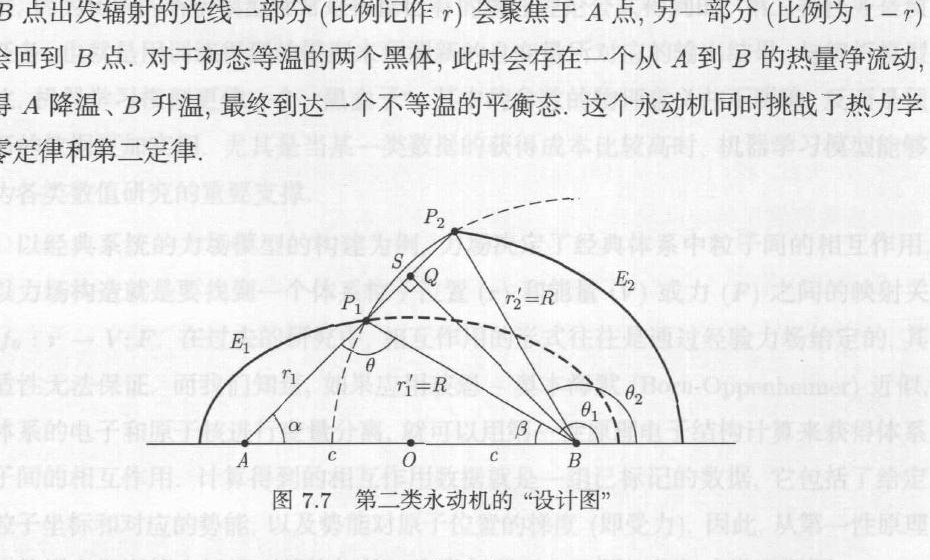
\includegraphics[width=0.78\linewidth]{figures/fig7_7_engine.png}
\caption{第二类永动机的“设计图”}
\label{fig:perpetual-motion}
\end{figure}

\begin{enumerate}[label=\arabic*.,leftmargin=2em]
\item 以上论述中存在一个明显的漏洞，指出它。
\item 选取几何参数。令小椭球的半长轴为 $a_1=2.5$，偏心率 $e=0.9$，球半径与小椭球半长轴之比为 $R/a_1=0.9$。设定两个黑体为有限大小的球体，半径为 $R_A=R_B=0.2$。试编写程序，对于任意从黑体上某一点发射的光线，都能给出其在到达某一个黑体之前的运动轨迹。随机选取几个初始条件并作图，以展示你的程序的可靠性。
\item 利用 Monte Carlo 方法或者其他任意你喜欢的积分方法进行统计，从 $A$ 出发的光线有多大比例回到了 $A$，多大比例到达了 $B$？对于 $B$ 而言呢？达到平衡态时两黑体的温度之间是什么关系？
\item 考虑两黑体不等半径的情形，取 $R_A=0.1,R_B=0.2$，重复上一问的讨论。
\item 不断减小两黑体的半径，检验热力学第二定律对于任何有限大小的黑体球都成立。
\end{enumerate}

% R23 extends through source scan p.297 / printed p.282, completing Chapter 7.
